\documentclass{article}
\usepackage[utf8]{inputenc}
\usepackage[a4paper, margin=1in]{geometry}
\setlength{\headheight}{23pt}
\usepackage{multicol}
\usepackage{fancyhdr}
\usepackage{listings}
\usepackage{amsmath}
\usepackage{float}
\usepackage{parcolumns}
\usepackage{caption}
\usepackage{graphicx, subfigure}

\title{EECS 570 Cheat Sheet}
\author{khtaur }
\date{February 2022}

\pagestyle{fancy}
\fancyhf{}
\fancyhead[R,RO]{Ke-Haur Taur\\khtaur@umich.edu}
\fancyhead[L,LO]{University of Michigan\\EECS 570 W22}
\fancyhead[C]{Parallel Computer Architecture\\Concept Cheat Sheet}
\fancyfoot[C]{\thepage}
\fancyfoot[L]{Ke-Haur Taur}
\renewcommand{\headrulewidth}{1pt}
\renewcommand{\footrulewidth}{1pt}

\begin{document}

\begin{multicols*}{2}

\section{Performance Measures}
Work and Depth (Add figure) \\
Amount of parallelism is Work/Depth
\subsection{Related theorems}
\subsubsection{Work Law}
You cannot avoid work by parallelizing:
$$\frac{T_1}{P} \leq T_p$$
\subsubsection{Depth Law}
More resources should make things faster:
$$T_\infty \leq T_p \text{(Best possible time)}$$
\subsubsection{Maximum Speedup}
Speedup is bounded by available parallelism:
$$\frac{T_1}{T_p} \leq \frac{T_1}{T_\infty}$$
Greedy scheduler achieves $T_p \leq \frac{T_1}{P} + T_\infty = 2T_p$

\section{Programming Models}
\subsubsection{Message Passing problems}
Process creation is external to execution environment
send and receive semantics (2-62, 2-63)
HW/SW POV.

\subsubsection{Shared memory problems}
(Figure in 2-70) Synchronization is hard. Implicit communication could introduce bugs and is hard to optimize.

\section{Vector operations}
\subsection{Vector masks and predication}
A predicate is a Boolean value used by an instruction to control whether the instruction is allowed to modify the architectural state or not. SIMD ISAs in vector processors apply one bit of a conditional mask Vector to the corresponding elements in the processed Vector registers.

\begin{lstlisting}[
    caption={Vector Processing and Predication},
    language=C++, 
    basicstyle=\footnotesize
]

parallel_for (i=0; i<n; i++) {
    if (cmask[i]){
        // dosomething
    }
    else{
        // dosomethingelse
    }
}

\end{lstlisting}

\subsection{Scatter stores and Gather loads}
This is used when the nature of the application does not cooperate with this row-by-row memory structure

\section{GPU Architecture}
\subsection{SIMT vs SIMD}
\begin{itemize}
    \item SIMD: A single thread of execution with a single program counter. Within this execution thread, individual SIMD instructions operate on wide vector registers.
    \item SIMT: Multiple independent threads each with its own independent program counter. The hardware aligns several of these threads in a warp and executes them in lock-step to improve efficiency.
\end{itemize}
\subsection{Logical hierarchy}
\begin{itemize}
    \item \textbf{Threads} are finest granularity and is selected by block to operate on data
    \item \textbf{Blocks} are group of threads which execute together in a batch
    \item \textbf{Grid} set of blocks which together execute the GPU operation
\end{itemize}

\subsection{Physical hierarchy}
\textbf{SM} can execute more than one block at any given time. If the SM has the resources available (registers and shared memory) then it will take on additional blocks. A SM scheduler schedules warps in which the warp decodes and issues instructions. (6-13)
\medskip\par\noindent
\textbf{Warps} are a set of N (usually 32) threads (if you have 128 threads in a block then threads 0-31 will be in one warp)
\medskip\par\noindent
\textbf{Threads} within a warp are bound and execute the same instructions. Threads within a warp fetch data from the memory together, so if you can ensure that all threads fetch data within the same 'segment' then you will only pay one memory transaction.

\subsection{Mapping logical to physical units}
\textbf{Blocks} will start on one SM and will remain there until it has completed. Once block is completed and retired and another block can be launched on the SM.

\subsection{Handling Nested Control Flow}
A SIMT execution model presents the programmer with the abstraction that individual threads execute completely independently and is achieved with a \textbf{SIMT stack}. 
\medskip\par\noindent
How does GPUs enable threads within a warp to follow different paths while employing a SIMD datapath that allows only one instruction to execute per cycle? Serialize execution of threads following different paths within a given warp using a \textbf{SIMT stack}.

\begin{itemize}
    \item \textbf{Wrap encounters branch}: Push join entry containing re-converge PC and execute one of two divergent paths while setting respective active masks. The other divergent entry is then pushed.
    \item \textbf{Wrap reaches last pipeline stage}: Pop entry off stack if wrap's next PC is identical to the re-converge PC.
\end{itemize}

\subsubsection{Deadlocks and SIMT stacks}
Locks and SIMT can cause deadlocks when combined. Consider the following program: lock-release is never reached since re-convergence is prohibited by a held lock.

\begin{lstlisting}[
    caption={SIMT stack deadlock},
    language=C++, 
    basicstyle=\footnotesize
]
void deadlock() {
    // 0 is denoted as unlocked
    // 1 is denoted as locked
    int *lock = 0;
    // (See CAS in 5.2.4)
    // Spin if CAS fails
    while(!CAS(lock, 0, 1)){};
    // ---------------
    // Critical Section
    // ---------------
    release(lock, 0);
}
\end{lstlisting}

\subsection{Issuing Fetched Instructions}
A structure for detecting intra-instruction dependencies is required. Straight-forward scoreboards are simple but requires way too much space (1 write-to bit per register; instructions with destination/source registers with bit set are stalled). 
\medskip\par\noindent
An alternative design is to record registers that would be written-to by \textbf{issued} instructions per warp.
\begin{itemize}
    \item After fetching an instruction: Set matching bits if source/destination registers match scoreboard entry of the warp.
    \item When instruction is ready for write-back: Clear the corresponding dependency entry in the scoreboard.
\end{itemize}

\subsection{$\mu$-arch Subtleties}
\subsubsection{Operand Collector}
The collector units are a way to space register operand accesses out in time so that no more than one access to a bank occurs in a single cycle. 
\medskip\par\noindent
When an instruction is received from the decode stage and a collector unit is available it is allocated to the instruction and the operand, warp, register identifier and valid bits are set. In addition, source operand read requests are queued in the arbiter. To simplify the design, data being written back by the execution units is always prioritized over read requests. The arbitrator selects a group of up to four non-conflicting accesses to send to the register file. To reduce crossbar and collector unit area the selection is made so that each collector unit only receives one operand per cycle.
\medskip\par\noindent
As each operand is read out of the register file and placed into the corresponding collector unit, a “ready bit” is set. Finally, when all the operands are ready the instruction is issued to a SIMD execution unit.

\subsubsection{Hiding Stalls}
Hiding stalls (4) latency hidden due to faster context switch made possible by larger RFs.

\subsection{Memory Hierarchy}
\subsubsection{Constant and Texture memory}
Constant memory is optimized for broadcast, i.e. when the threads in a warp all read the same memory location.
Texture memory addressing has 2D and 3D locality, so cache line fills pull in 2D and 3D blocks of memory instead of rows

\section{Synchronization}
\subsection{Waiting algorithms}
\subsubsection{Spin}
Repeatedly waits and lower overhead but wastes CPU resource.
\subsubsection{Block}
Suspends waiting and higher overhead but CPU can do other things.

\subsection{Atomic R/W and locks}
\subsubsection{Test and Set}
Test and Set is both a read and write; spinning causes lots of in-validations.
\begin{lstlisting}[
    caption={Test and set},
    language=C++, 
    basicstyle=\footnotesize
]
bool TestAndSet(bool* lock) {
    // Test
    bool initial = lock;
    // Set
    &lock = true;
    return initial;
}

void critical(int *lock) {
    while (TestAndSet(&lock) == 1);
    // only 1 thread can be in here
    // ---------------
    // critical section
    // ---------------
    // release lock
    &lock = 0;
}
\end{lstlisting}

\subsubsection{Test and Test and Set (TTS)}
TTS in an invariant of T\&S. It gates the thread from T\&S if first test fails. All the processors attempt to load lock upon release, and likely try to T\&S the block and causes a storm of coherence traffic, clogs things up badly. Most importantly, it is still unfair.
\begin{lstlisting}[
    caption={Test and Test and set},
    language=C++, 
    basicstyle=\footnotesize
]
void critical(int *lock) {
    lock_val = &lock;
    while (true) {
        // Test on local copy
        if (lock_val == 0) {
            // And Test and Set
            while (TestAndSet(&lock) == 1);
            // only 1 thread can be in here
            // ---------------
            // critical section
            // ---------------
            // release lock
            &lock = 0;
        }
    }
}
\end{lstlisting}

\subsubsection{Fetch and in/decrement (FAI)}
This instruction is used to construct ticket-based locks. Since many threads might ask for a lock at the same time, the FAI instruction must be atomic to maintain correctness.
\medskip\par\noindent
Ticket based locks can never cause multiple RMWs since only the next ticket holder is able to acquire the lock.
\medskip\par\noindent
However, if threads consume an average of k $\times$ base time per critical section, the calling thread can be expected to probe the global \texttt{lock.turn} about k times.

\begin{lstlisting}[
    caption={Ticket locks with FAI},
    language=C++, 
    basicstyle=\footnotesize
]
int FAI(int location, int inc) {
    int value = *location
    *location = value + inc
    // Returns original value
    return value
}

struct locktype {
    int tickets,
    int turn
}

void Lock(locktype* lock) {
    // FAI returns pre-increment value
    // Stores incremented value in memory
    int myturn = FAI(&lock.tickets)
    
    // Probes global lock.turn indefinitely
    while lock.turn != myturn
        // spin until lock is acquired
        continue;
}

void UnLock(locktype* lock) {
    // This
    FAI(&lock.turn)
    // Or this?
    &lock.turn++;
}
\end{lstlisting}

\subsubsection{Compare and Swap}
CAS checks that the contents of the location match the expected value. If so, it replaces them with the new value, but if not it has no effect. In any case, the previous value of the variable is returned. The CAS instruction takes three parameters: a location, an "expected value" for that location, and a new value for the location.

\begin{lstlisting}[
    caption={Compare and Swap},
    language=C++, 
    basicstyle=\footnotesize
]
bool CAS(int *loc, int expt, int new){
    // Compare
    if &loc != expt {
        // loc is modified!
        // CAS failed
        return false;
    }
    // Swap
    &loc = new;
    return true
}

void critical (int *x) {
    // Expecting 0 means no lock
    // Thread 1 identified as 1
    while (!CAS(&x, 0, 1)) {
        continue;
    }
    // ---------------
    // Enter critical section
    // ---------------
}
\end{lstlisting}

\medskip\par\noindent
CAS is also used to build MCS queue based locks. CAS is specifically used when a node tries to release and see if their are no successors. In this case, CAS expects the tail of the list to be null; if CAS fails, the releasing node spins till successor is known.

\begin{lstlisting}[
    caption={MCS locks with CAS},
    language=C++, 
    basicstyle=\footnotesize
]

class lock{
    public:
        node* tail = null;
    
    acquire(node* p){
        p->next = null;
        p->wait = true;
        
        // Make queuing node
        // the last node in list
        // The swap Op is fenced
        node* prev = swap(&tail, p);
        // If queue is not empty
        if (prev != null){
            prev->next = p;
            // Spin till prev unlocks
            while (p->wait){};
        }
    }
    
    release(node* p){
        node* succ = p->next;
        if (succ == null){
            // Check if acquire happened
            // after loading p->next
            if (CAS(&tail, p, null)){
                return;
            }
            // CAS fails;
            // spin till successor known
            while (p->next != null){};
            succ = p->next;
        }
        succ->wait = false;
    }
}

\end{lstlisting}

\subsection{Load-locked Store-conditional}
LL and SC are a pair of instructions used in multithreading to achieve synchronization. Load-locked returns the current value of a memory location, while a subsequent store-conditional to the same memory location will store a new value only if no updates have occurred to that location since the load-link. Together, this implements a lock-free atomic read-modify-write operation.
\medskip\par\noindent
If any updates have occurred, the store-conditional (SC) is guaranteed to fail, even if the value read by the load-link has since been restored. As such, an LL/SC pair is stronger than a read followed by a compare-and-swap (CAS), which will not detect updates if the old value has been restored (see ABA problem).
\medskip\par\noindent
SC also fails when finding that the flag is cleared caused by invalidation, cache evictions or context switches.

\begin{lstlisting}[
    caption={Load-locked Store Conditional},
    language=C++, 
    basicstyle=\footnotesize
]

void lock(int *lock) {
    while(true){
        // load-locked
        ll(r1, lock);
        // 0 if lock no holder
        if(r1 == 0){
            // Update holder
            r2 = r1;
            // fail store-cond
            if(sc(r2, lock)){
                break;
            }
        }
    }
}

void unlock(int *lock) {
    lock = 0;
}
\end{lstlisting}

\subsection{Barriers}

\section{Transactional Memory}
\subsection{Motivation}
Explicit locking breaks program abstraction and is possible to deadlock.

\begin{lstlisting}[
    caption={How to do this?},
    language=C++, 
    basicstyle=\footnotesize
]

// Before and after calling transfer()
// k is exclusively in set S1 or S2
void transfer(set S1, set S2, Key k) {
    atomic {
        delete(S1, k);
        insert(S2, k)
    }
}
\end{lstlisting}

\subsubsection{Why is syncing with locks hard?}
\begin{itemize}
    \item Locks too fine: High overhead
    \item Locks too coarse: Poor scalability
\end{itemize}
Similar to transaction speculatively execute critical sections, \textbf{lock elision} is based on the premise that various critical sections access disjoint data.

\subsection{Abstraction}
Semantics contain no locks and critical sections are executed speculatively.

\subsection{Begin/End of Tx}
\begin{itemize}
    \item Begin:
    \begin{itemize}
        \item Create register checkpoint for rollback
        \item Track loaded addresses (remember read addresses)
        \item Buffer all stores (invisible to other threads)
    \end{itemize}
    \item End:
    \begin{itemize}
        \item Check if read set is touched
        \item Commit if read set is clean; otherwise abort and restore checkpoint
    \end{itemize}
\end{itemize}


\subsection{Components}
\subsubsection{Read/Write Sets}
Set of shared addresses critical section reads/writes

\subsubsection{Version Management}
\begin{itemize}
    \item Lazy:
    \begin{itemize}
        \item Add store addresses to write table
        \item Load from write table if address present; read from memory otherwise
        \item Commit all writes in table to memory and clear table (Slow)
        \item Clear table upon discovering conflicts (Fast)
    \end{itemize}
    \item Eager:
    \begin{itemize}
        \item Stores update write log and add to write set; All stores write directly to memory
        \item Load directly from memory
        \item Commits are made during stores; nothing is required (Fast)
        \item If discovered conflicts, roll back according to write log (Slow)
    \end{itemize}
\end{itemize}

\subsubsection{Conflict Detection}
\begin{itemize}
    \item Lazy:
    Easier with STM and so are transactions with a large footprint (touches lots of different addresses that probably couldn't fit in a cache). This is because STM is usually implemented by the OS at page granularity.
    \begin{itemize}
        \item Only adds to read/write set upon load or store
        \item Upon commit, for every address in write set, check if address is in read set of other threads
    \end{itemize}
    \item Eager:
    Easier to do with small transactions and usually implemented as HTM.
    \begin{itemize}
        \item Also check other threads read/write set for conflicts for every read/write
        \item Just clear read/write sets upon commit
    \end{itemize}
\end{itemize}

\section{Cache Coherence}
\subsection{Invariants}
\begin{itemize}
    \item \textbf{SWMR}: There is either one writer or zero or more readers of a cache line at any (logical) time.
    \item \textbf{Data Value Invariant}: All cores see cache line updates in the same order. (e.g., if Core 1 observes data X go from $0 \rightarrow 1 \rightarrow 3$, then all other cores must observe this sequence of updates as well)
\end{itemize}
\subsection{Snooping Bus}
All caches monitor/snoop the bus for messages and bus is point of serialization. 

\subsubsection{Snooping Cache Controller}
There are some implementation considerations. Tags in caches are often multi-ported for CPU and cache controller to concurrently access tags. And memory will still assume that sharers exist since it is not notified when blocks silently evict.
\begin{itemize}
    \item How to report snoop results? Requires shared/dirty signals to indicate if shared copies exist or if block is dirty. If block is shared, an arbitration scheme is needed for the sharer to supply data to requester.
    \item When does memory provide data to requester? Either wait for fixed cycles or all caches respond that they do not hold shared data.
    \item Handling write-backs without penalty? A victim buffer stores evicted lines and handles relevant snoop transactions and maintaining write/read order.
\end{itemize}

\subsubsection{Snooping with Multiple Level Caches}
Cache inclusion allows for easier snooping with multi-level caches (Data in L1 must be in L2). However cases where line is evicted in L2 but not in L1 requires back invalidation.
\medskip\par\noindent
Consider L1 is 2-Way and L2 is 4-Way and the CPU emits the following access patterns that all match to the same set: ABACADAE.
\medskip\par\noindent
Since notion of LRU is local to each cache level, the insertion of E to L2 evicts A (L2 view of LRU), which requires L1 to evict A in order to respect inclusion. The reason LRU is local is because various levels have different cache access streams.

\subsubsection{Snooping with Split-Tx Bus}
A split transaction bus allows for simultaneous transactions but requires (1) handling conflicting transactions to same block, (2) control requests/responses to prevent deadlock and (3) correctly ordering snoop responses.
\medskip\par\noindent
A \textbf{deadlock} example is that Core 2 (C2) see's that the latest clean line is at C1 and sends a request (R) directly to the request/response queue of C1. Before C1 responds to C2, it is waiting for a particular response (P). If P arrives at the queue after R then C1 is unable to process R since R is in front of P in the queue.
\medskip\par\noindent
A \textbf{livelock} example is that both C1 and C2 issue a \texttt{GetM} request to the same location. If C1 sees the invalidation of \texttt{GetM} before doing anything, C1 aborts its store and allows C2 to process its store. If C1 issued a same \texttt{GetM} request before C2 finishes its store, the situation ping-pongs between the two cores and is live-locked.
\medskip\par\noindent
A \textbf{starvation} example is that C1 issues a \texttt{GetS} request and C2 issues a \texttt{GetM} to the same location. If C1 sees the invalidation of \texttt{GetM} before the \texttt{GetS} data response, C1 throws the data away and allows C2 to process its store. If this access pattern continues, C1 will not be able to make forward progress due to unfair arbitration.

\subsubsection{TLB Coherence/Shootdown}
TLBs are itself a per-core cache (every core has its own TLB). TLB entries need to be in sync with their respective page table entries (PTE) at all times. Whenever a PTE is modified by any of the cores, that particular TLB entry is invalidated in all of the cores instructed by the OS.

\subsection{State Characteristics}
\begin{itemize}
    \item Modified  – the only copy; writable; dirty
    \item Exclusive – the only copy; writable; clean
    \item Owned     – shared, but dirty; only one owner
    \item Shared    – shared; read-only; clean
\end{itemize}

\subsubsection{Modified state motivation}
Starting with the valid/invalid protocol for write-through caches. Adding "ownership" state allows for \textbf{mutual exclusion or multiple sharers}.

\subsubsection*{Update or Invalidate?}
\begin{itemize}
    \item Invalidation is bad for single producer multiple consumers
\end{itemize}

\subsubsection*{Coherence Decoupling}
Keep stale data after invalidation. Sends out a load in parallel and compare with kept value to confirm speculation. Solves \textbf{false sharing} and addresses \textbf{silent stores} (Writing back same values).

\subsubsection{Exclusive state motivation}
Adding an exclusive state alleviates overhead of frequent read-upgrade sequences (e.g., $I \rightarrow S \rightarrow M$), causing less traffic. Transitions to Modified state when data is dirty.

\subsubsection{Owned state motivation}
Modified state downgrades \textbf{must} write-back to memory and waste bandwidth. Owned state only writes back to memory when releasing ownership.

\subsubsection{Common Sharing Patterns}
\begin{itemize}
    \item \textbf{Code/Read-only objects:} Invalidations are minimal since they will not be written to.
    \item \textbf{Migratory/Frequently-written objects}: Working set is invalidated before it can grow to a large size. (e.g., Core 1 does a read and write then Core 2 subsequently does the same thing.)
    \item \textbf{Synchronization objects}: Depend on the nature of the program. (T\&S will not result in many invalidations if contention is low.)
\end{itemize}


\subsection{Directory Coherence}
Directories store owner and sharer information of each cache line. Instead of broadcasting, processor sends coherence events to the directory instead.

\subsubsection{Centralized or Distributed?}
Centralized directories are not scalable to overwhelming traffic but distributing directories can no longer serialize accesses from all addresses. Distributed directories are assigned partitions from contiguous memory.

\subsubsection{Why Distributed?}
The hypothesis is that invalidations caused by writes to a shared location is typically small. Distributed directories behave similarly to snooping protocols if data is shared across many cores.

\subsubsection{Directory Composition}
All lines contain the state of the block, pointer to the owner and a sharers list. Each have considerable design space.
\begin{itemize}
    \item \textbf{State Representation}: Though there are only few stable states, but a large amount of transient states are required to ensure coherence.
    \item \textbf{Maintaining Sharers List}: Though most blocks are only cached in less than 4 nodes but there are instances where a block is shared in many caches. We could either use (1) a bit vector, (2) limited pointers which requires force invalidations when shares exceed the fixed amount or (3) linked lists where each node pointers to the next/previous sharer.
    \item \textbf{How accurate is our sharer list?} With clean eviction notification, we don't falsely invalidate blocks. But we will evict read-only data due to limited space and introduced messages will introduce complications to transient states
    \item \textbf{Where is our sharer list?} Consider that caches only store a small portion of data, only those pieces of data are to be maintained by the directories. Anything not in the directory cache is invalid and should be invalidated in all caches if existent.
\end{itemize}

\subsubsection{Possible Races}
\begin{itemize}
    \item \textbf{Writeback \& Read}: Local node evicts dirty copy to memory (\texttt{PutM}), but Remote node reads the same line (\texttt{GetS}). 
    \begin{itemize}
        \item \textbf{The GetS request reaches the directory before the PutM} and still think that Local is the owner; Directory in response sends a FwD-GetS to Local which detects a race. The line in local transitions from $MI^A$ to $SI^A$ while sending the data to Remote.
    \end{itemize}
    \item \textbf{Read \& Write}: Local node requests a load (GetS) and Remote requests a store (GetM) \textbf{after} the directory sends out the data to Local and invalidations from GetM arrives at Local before the requested line.
    \begin{itemize}
        \item Local transitions from $IS^{AD}$ to $IS^{AD}I$ and does one load then transitions to invalid while sending a Inv-Ack to Remote.
    \end{itemize}
\end{itemize}



\section{Memory Organization}
\subsection{Nomenclature}
\begin{itemize}
    \item UMA: Main memory access latency for every core is identical
    \item NUMA: Individual memory is closer to nodes. Data placement is non-trivial.
    \item COMA: Data will migrate to where its used. When a processor requests a block from a remote memory, the block is inserted in both the processor’s cache and the node’s AM. A block can be evicted from an AM if another block needs the space. The processor dynamically attracts its working set into its local memory module. The data the processor is not accessing overflows and is sent to other memories. Other COMA derivations include:
    \begin{itemize}
        \item Flat-COMA: A memory distributed and fixed directory redirects the request to another node if the home does not have a copy of the block.
        \item Simple-COMA:
        \item Reactive-COMA: OS sees number of refetches (access that brings in a block that was displaced from local memory) issued by a node to blocks of a page
    \end{itemize}
\end{itemize}

\section{Memory Consistency}

\subsection{Coherence and Consistency}
Coherence concerns only one memory location while Consistency concerns programmer-visible ordering for all locations.

\subsection{Program Order Relaxations}

\noindent\begin{minipage}{.2\textwidth}
\captionsetup{labelformat=empty}
\begin{lstlisting}[
    caption=core 1,
    frame=tlrb, 
    basicstyle=\footnotesize
]{Name}
i1 A = 1;
i2 flag = 1;
\end{lstlisting}
\end{minipage}\hfill
\begin{minipage}{.2\textwidth}
\captionsetup{labelformat=empty}
\begin{lstlisting}[
    caption=core 2,
    frame=tlrb,
    basicstyle=\footnotesize
]{Name}
i3 while(!flag);
i4 print(A)
\end{lstlisting}
\end{minipage}
\captionof{lstlisting}{Message Passing Litmus test}

\noindent\newline
It is possible for core 2 to see core 1's write to \texttt{flag} before write to \texttt{A}. Out-of-Order execution or coalescing store buffer in core 1 may re-order writes. The only forbidden case in SC is for \texttt{flag} to be 1 and \texttt{A} is 0 since $i3$ and $i4$ reordering is forbidden in SC (See 9.5).

\subsection{Store Atomicity}
New values might not reach all nodes at the same time any might trigger unexpected results. We say that store stomicity is relaxed if the ordering mechanisms are not strong enough to forbid certain outcomes. Consider the following write-to-read causality (WRC) litmus test: The write to A causes B to be set to 1.

\noindent\begin{minipage}{.15\textwidth}
\captionsetup{labelformat=empty}
\begin{lstlisting}[
    caption=core 1,
    showlines=true,
    frame=tlrb, 
    basicstyle=\footnotesize
]{Name}
A = 1;
 
\end{lstlisting}
\end{minipage}\hfill
\begin{minipage}{.15\textwidth}
\captionsetup{labelformat=empty}
\begin{lstlisting}[
    caption=core 2,
    frame=tlrb,
    basicstyle=\footnotesize
]{Name}
while(A == 0);
B = 1;
\end{lstlisting}
\end{minipage}\hfill
\begin{minipage}{.15\textwidth}
\captionsetup{labelformat=empty}
\begin{lstlisting}[
    caption=core 3,
    frame=tlrb,
    basicstyle=\footnotesize
]{Name}
while(B == 0);
print(A)
\end{lstlisting}
\end{minipage}
\captionof{lstlisting}{When does core 2/3 see A=1?}

\noindent\newline
It is possible to print $A == 0$: (1) A=0 initially cached at core 3 in shared state. (2) Update for A arrives at core 2 and sends out B=1. (3) Update for B arrives at core 3 and core 3 prints A=0 before invalidation from core 1 arrives.
\medskip\par\noindent
Another case for this to happen is if cores 1 and 2 share an intermediate store buffer for simultaneous multi-threading purposes. It is possible to print $A==0$ if the store buffer retires the write to B and not A.
\medskip\par\noindent
One optimization that relaxes store atomicity is the post-retirement store buffers. When a store miss occurs, the value to store is pushed into the store buffer and subsequent loads can read from the store buffer instead of waiting for the store miss to be serviced. This hides latency of store misses while stores/loads are still ordered w.r.t. other stores/loads. However this breaks Dekker's algorithm: if the write to $A=1$ and $B=1$ store misses are not yet serviced (memory thinks they are both 0) then both cores proceed to critical sections when values of $A$ and $B$ being 0.

\subsection{Dependence Order}
Consider the following stream of instructions:
\begin{lstlisting}[
    caption=Dependent instructions,
    frame=tlrb,
    basicstyle=\footnotesize
]{Name}
# Dependent instructions
i1 ld  r1, [0x1]
i2 add r2, r1, 4
i3 ld. r3, [r2]

# False Dependencies
i4 ld  r4, [0x2]
i5 xor r5, r4, r4
i6 ld. r6, [r5+4]
\end{lstlisting}

\noindent
It would make sense to maintain original ordering between these instructions to maintain correctness. Some specifications even maintain ordering for false dependencies. Dependence order captures what an out-of-order core is allowed to do.

\noindent\newline
The following are cases that are considered to have dependence order:
\begin{lstlisting}[
    caption=Dependent order programs,
    frame=tlrb,
    basicstyle=\footnotesize
]{Name}
# Exec of Y (r2) is conditional on
# X (r1) and Y is a store
ld  r1, [0x1]
bne next, r1
st  r2, [r1]
# Dependent instructions
ld  r1, [0x1]
add r2, r1, 4
ld  r3, [r2]
\end{lstlisting}

\subsection{Sequential Consistency}
Consider the Store Buffering (SB) litmus test

\noindent\begin{minipage}{.2\textwidth}
\captionsetup{labelformat=empty}
\begin{lstlisting}[
    caption=core 1,
    frame=tlrb, 
    basicstyle=\footnotesize
]{Name}
i1 st 1,  x;
i2 ld r1, y;
\end{lstlisting}
\end{minipage}\hfill
\begin{minipage}{.2\textwidth}
\captionsetup{labelformat=empty}
\begin{lstlisting}[
    caption=core 2,
    frame=tlrb,
    basicstyle=\footnotesize
]{Name}
i3 st 1,  y;
i4 ld r2, x;
\end{lstlisting}
\end{minipage}
\captionof{lstlisting}{Store Buffering litmus test}

\noindent\newline
Sequential consistency requires that the interleavings respect the program order within each thread. In this case, $i1$ must happen before $i2$ and $i3$ must happen before $i4$. The case where r1 and r2 both equal to 0 is forbidden.
\medskip\par\noindent
Another important test is Dekker's algorithm (store buffer litmus test): it checks if 2 cores can enter a critical section at the same time.

\noindent\begin{minipage}{.2\textwidth}
\captionsetup{labelformat=empty}
\begin{lstlisting}[
    caption=core 1,
    frame=tlrb, 
    basicstyle=\footnotesize
]{Name}
A = 1;
while(B != 0);
// Critical Sec.
\end{lstlisting}
\end{minipage}\hfill
\begin{minipage}{.2\textwidth}
\captionsetup{labelformat=empty}
\begin{lstlisting}[
    caption=core 2,
    frame=tlrb,
    basicstyle=\footnotesize
]{Name}
B = 1;
while(A != 0);
// Critical Sec.
\end{lstlisting}
\end{minipage}
\captionof{lstlisting}{Dekker's Algorithm (SB litmus test)}

\noindent\newline
The only case where both cores enter the critical section is that the load to A and B happens before the store to A and B, which violates sequential consistency.

\subsubsection{SC HW Perspective}
Strict ordering is required so the SC MCM precludes OoO CPUs. This essentially conflicts with latency hiding techniques.

\subsubsection{SC SW Perspective}
Most programmers use libraries for synchronization hence, they don’t actually need SC guarantees.

\subsubsection{SC Compiler Perspective}
No memory ops may be reordered which basically disallows Register allocation and other optimizations. Conflict analysis can determine the minimal set of delays to enforce SC.

\subsection{Total Store Order}
Store buffers mentioned in write atomicity is allowed. There is no store to load enforced ordering; however, Dekker's algorithm would fail. Loads return the most recent value w.r.t. memory order ($<_M$) and w.r.t. local program order ($<_P$).

\subsubsection{TSO SW Perspective}
TSO ISAs provide an STBAR (store barrier) to manually force order. A RMW would naturally respect TSO orderings since nothing can be reordered across the \texttt{acquire} (essentially a annotated load) and \texttt{release} (essentially a store).

\subsubsection{TSO HW Perspective}
TSO allows a FIFO-ordered, non-coalescing store buffer and buffer is drained on RMW and STBAR operations. Coalescing only allowed for adjacent stores to same block. In this case, a STBAR enforces the store to be visible to all cores before proceeding. 
\medskip\par\noindent
In other words, TSO by default allows a core to read its write early (from the core's own store buffer) but a core is not allowed to read writes from other cores early (Also known as multiple copy atomic -- MCA). Processor consistency (PC) relaxes store atomicity and allows some cores to see writes before other cores (nMCA).

\subsection{Partial Store Order}
Adds a relaxed formal requirement such that stores are ordered only if they are separated by
a memory barrier and Stores to the same address are still ordered.

\subsubsection{PSO HW Perspective}
Out of order execution without speculation is still not allowed because load to load/store ordering is still enforced.

\subsection{Relaxed Memory Order}
Basically follows dependence ordering with the prior instruction being a load. Stores to same addresses are performed in program order. Note that RMO does not preserve same addresses load-to-load orderings.

\subsubsection{RMO SW Perspective}
Programmers are responsible to place fences where needed. Specifying minimum amount of barriers is hard. The only constraint of the compiler is to not reorder stores to same addresses.

\subsubsection{RMO HW Perspective}
Allows unordered coalescing post-retire store buffers like PSO. Hardware is able to achieve OoO with fence ISA implementations by stalling instructions from issuing when fence is at the head of ROB.

\subsection{Weak Ordering}
Only specify/annotate instructions with sync operations such that the entire programs would behave like SC. But the compiler is free to reorder any instructions except across sync borders.

\subsection{Release Consistency}
Acquires and releases in RC only say that instructions within (critical section) are not allowed to be reordered. Instructions before the acquire and after the release are allowed to be reordered in the critical section (roach-motel movement). Instructions after the acquire (i2, i3 and i4) should happen after the acquire. Releases enforce ordering preceding it (i1, i2 and i3 are done when executing to the release). In other words, i1 cannot cross the release and i4 cannot cross the acquire.
\begin{lstlisting}[
    caption=Release consistency orderings,
    frame=tlrb,
    basicstyle=\footnotesize
]{Name}
i1 st r1, [0x1]
acquire
i2 st r2, [0x2]
i3 st r3, [0x3]
release
i4 st r4, [0x4]
\end{lstlisting}

\subsubsection{RCsc and RCpc}
In RCsc, special accesses (\texttt{acq} and \texttt{rel}) are sequentially consistent whereas in RCpc, they are processor consistent (reserve $<_P$ except for store-to-loads while relaxing store atomicity).

\noindent\begin{minipage}{.2\textwidth}
\captionsetup{labelformat=empty}
\begin{lstlisting}[
    caption=core 1,
    frame=tlrb, 
    basicstyle=\footnotesize
]{Name}
i1 rel st 1,  x;
i2 acq ld r1, y;
\end{lstlisting}
\end{minipage}\hfill
\begin{minipage}{.2\textwidth}
\captionsetup{labelformat=empty}
\begin{lstlisting}[
    caption=core 2,
    frame=tlrb,
    basicstyle=\footnotesize
]{Name}
i3 rel st 1,  y;
i4 acq ld r2, x;
\end{lstlisting}
\end{minipage}
\captionof{lstlisting}{Annotated Store Buffering litmus test}

\noindent\newline
With RCsc, the order $i1$ to $i2$ and $i3$ to $i4$ is maintained; hence the situation of r1 and r2 both being 0 is disallowed. Conversely, the order of $i1/i2$ and $i3/i4$ is not maintained in RCpc and the result of r1 and r2 both equal to 0 is observable.

\begin{lstlisting}[
    caption=Why RCpc?,
    frame=tlrb,
    basicstyle=\footnotesize
]{Name}
acquire A
// Crit. Sec. 1
release A
acquire B
// Crit. Sec. 2
release B
\end{lstlisting}

\noindent\newline
In RCpc, acquire B is allowed to cross critical section 1 (and release A) and be ordered after acquire A and release B is allowed to be reordered till after release A. This allows order of both critical sections 1 and 2.

\subsection{Data Races}
A program is racy if accesses to the same address on different threads where at least 1 is a store and at least 1 is not a sync access are not ordered by sync accesses.

\noindent\begin{minipage}{.2\textwidth}
\captionsetup{labelformat=empty}
\begin{lstlisting}[
    caption=core 1,
    frame=tlrb, 
    basicstyle=\footnotesize
]{Name}
i1 x = 1;
i2 y = 1; (Race)
\end{lstlisting}
\end{minipage}\hfill
\begin{minipage}{.2\textwidth}
\captionsetup{labelformat=empty}
\begin{lstlisting}[
    caption=core 2,
    frame=tlrb,
    basicstyle=\footnotesize
]{Name}
i3 r1 = y; (Race)
i4 z  = 1;
\end{lstlisting}
\end{minipage}
\captionof{lstlisting}{Race example 1}

\noindent\newline
Even in SC, the example with no annotations would constitute a race: $i2$ and $i3$ can be reordered. But if $i2$ is labeled as a release and $i3$ is labeled as an acquire, then r1 would be 1 given RCsc.

\noindent\begin{minipage}{.2\textwidth}
\captionsetup{labelformat=empty}
\begin{lstlisting}[
    caption=core 1,
    showlines=true,
    frame=tlrb, 
    basicstyle=\footnotesize
]{Name}
i1 x = 1;
i2 y = 1; (Race)



\end{lstlisting}
\end{minipage}\hfill
\begin{minipage}{.24\textwidth}
\captionsetup{labelformat=empty}
\begin{lstlisting}[
    caption=core 2,
    frame=tlrb,
    basicstyle=\footnotesize
]{Name}
next:
i3 r1 = y; (Race)
# Go back till y is 1
i4 bne r1, 1, next;
i5 r2 = x;
\end{lstlisting}
\end{minipage}
\captionof{lstlisting}{Race example 2}

\noindent\newline
Given RCsc and $i2$ is a release and $i3$ is an acquire, $i1$ is guaranteed to happen before $i2$. No cases remain such that they are not ordered by sync accesses.

\subsubsection{SC with annotated WO/RC}
If annotations to stores/loads (acquires/releases) are labeled correctly, one would get a SC program.

\noindent\begin{minipage}{.2\textwidth}
\captionsetup{labelformat=empty}
\begin{lstlisting}[
    caption=core 1,
    showlines=true,
    frame=tlrb, 
    basicstyle=\footnotesize
]{Name}
acquire L
st x,  2
ld r1, y
release L

\end{lstlisting}
\end{minipage}\hfill
\begin{minipage}{.24\textwidth}
\captionsetup{labelformat=empty}
\begin{lstlisting}[
    caption=core 2,
    frame=tlrb,
    basicstyle=\footnotesize
]{Name}
acquire L
ld r3, x
st z,  1
ld r2, x
release L
\end{lstlisting}
\end{minipage}
\captionof{lstlisting}{SC with annotated WO/RC}

\noindent\newline
Core 2 has no idea whether code within the acquire/release in core 1 is reordered; hence achieving data race free (DRF). Cores without the permissions (yet to acquire lock) cannot access variables locked by the core in question. Code in core 1 either happened before or after code in core 2

\section{Program Language MCM}
2 main ideas arise in a programming language MCM specification:
\begin{itemize}
    \item Programmers annotate memory accesses (data/sync) for compilers to recognize reordering optimizations.
    \item Programmers ensure DRF -- all bets are off if a program is racy.
\end{itemize}

\subsection{C++ Memory Model}
\texttt{Atomic} variables in C++ can be used for fine-grained synchronization. Most intuitive cases are SC atomics in C++. Only enforce synchronization when release is read by an acquire. Sequentially consistent loads are acquires and stores are releases.

\noindent\begin{minipage}{.22\textwidth}
\captionsetup{labelformat=empty}
\begin{lstlisting}[
    caption=core 1,
    language=C++,
    showlines=true,
    frame=tlrb, 
    basicstyle=\footnotesize
]{Name}
atomic <int> x;
atomic <int> y;
atomic <int> z;

// Relaxed store
x.store(1, relax);

// RCsc
y.store(1, sc);

// RCpc
z.store(1, rel);
\end{lstlisting}
\end{minipage}\hfill
\begin{minipage}{.22\textwidth}
\captionsetup{labelformat=empty}
\begin{lstlisting}[
    caption=core 2,
    language=C++,
    frame=tlrb,
    basicstyle=\footnotesize
]{Name}
/*
    Not an acquire!
    Won't snyc with
    acq or rel
*/
r1 = x.load(relax);

// RCsc load
r2 = y.load(sc);

// RCpc load
r3 = z.load(acq);
\end{lstlisting}
\end{minipage}
\captionof{lstlisting}{SC with annotated WO/RC}

\subsubsection{Data races in C++}
Consider the following where compiler optimizations would violate correctness. The following code consists of races due to missing synchronization annotations.
\begin{lstlisting}[
    caption=Races in C++,
    language=C++,
    frame=tlrb,
    basicstyle=\footnotesize
]{Name}
// Shared variable x
int i = x;

// Compiler optimization:
// Read x from memory; save stack space
if(i < 2){
    // foo:
    // x changed here by other core
    
    // Compiler optimization:
    // Switch implemented as jump table
    // and load i from x
    switch(i) {
        case 0:
        case 1:
        /*
            Dropped default case!
            Compiler deems it useless
        */
        default:
    }
}
\end{lstlisting}

\subsection{C++ atomics}
SC atomics have total order respected by all cores. Consider the independent read/write (IRIW) litmus test:

\noindent\begin{minipage}{.11\textwidth}
\captionsetup{labelformat=empty}
\begin{lstlisting}[
    caption=core 1,
    showlines=true,
    frame=tlrb,
    basicstyle=\footnotesize
]{Name}
A = 1;
 
\end{lstlisting}
\end{minipage}\hfill
\begin{minipage}{.11\textwidth}
\captionsetup{labelformat=empty}
\begin{lstlisting}[
    caption=core 2,
    frame=tlrb,
    showlines=true,
    basicstyle=\footnotesize
]{Name}
B = 1;

\end{lstlisting}
\end{minipage}\hfill
\begin{minipage}{.11\textwidth}
\captionsetup{labelformat=empty}
\begin{lstlisting}[
    caption=core 3,
    frame=tlrb,
    showlines=true,
    basicstyle=\footnotesize
]{Name}
r1 = A;
r2 = B;
\end{lstlisting}
\end{minipage}\hfill
\begin{minipage}{.11\textwidth}
\captionsetup{labelformat=empty}
\begin{lstlisting}[
    caption=core 4,
    frame=tlrb,
    showlines=true,
    basicstyle=\footnotesize
]{Name}
r3 = B;
r4 = A;
\end{lstlisting}
\end{minipage}
\captionof{lstlisting}{IRIW Litmus test}

\noindent\newline
The outcome of $r1=1; r2=0; r3=1; r4=0$ is not allowed with SC atomics but is allowed with acquire/release atomics due to nMCA of PC.

\subsubsection{Cumulative atomics in C++}
Acquire/release atomics in C++ is cumulative. Consider the following:

\begin{minipage}{.15\textwidth}
\captionsetup{labelformat=empty}
\begin{lstlisting}[
    caption=core 1,
    frame=tlrb,
    showlines=true,
    basicstyle=\footnotesize
]{Name}
// Code
x = 1;
// Code

\end{lstlisting}
\end{minipage}\hfill
\begin{minipage}{.15\textwidth}
\captionsetup{labelformat=empty}
\begin{lstlisting}[
    caption=core 2,
    frame=tlrb,
    showlines=true,
    basicstyle=\footnotesize
]{Name}
acq l1
// Code
r1 = x;
rel l1;
\end{lstlisting}
\end{minipage}\hfill
\begin{minipage}{.15\textwidth}
\captionsetup{labelformat=empty}
\begin{lstlisting}[
    caption=core 3,
    frame=tlrb,
    showlines=true,
    basicstyle=\footnotesize
]{Name}
// Sees rel



\end{lstlisting}
\end{minipage}
\captionof{lstlisting}{C++ cumulative atomics}

\noindent\newline
When core 3 sees the release made in core 2, it has to see the load ($r1=x$) before the release and the store before the load ($x=1$).

\noindent\newline
When a release is read by a data access, it is considered a data race; if read by a relaxed access, there is \textbf{NO} enforced synchronizations. However, conflicting relaxed accesses are not races.

\subsubsection{Mapping atomics to assembly}
In x86, \texttt{acq}/\texttt{rel} and relaxed atomics are mapped to regular loads and stores. (i.e., In TSO, \texttt{acq} is always before a \texttt{rel}) For SC atomics (RCsc), a \texttt{MFENCE} is required either after a store or before a load to protect store to load ordering in TSO.

\section{Prefetching and MCM}
There is still room of improving performance for SC by prefetching cache lines. The main point is to separate prefetching from actually performing the memory operation. It is like preventing a miss when actually trying to perform the operatin in program order. If the prefetched line is invalidated, we have to request for the line again before committing. Thing to note is that this optimization is done in hardware only; the compiler does not add any additional loads.

\subsection{Prefetching in R10K}
The R10K allows load operations to speculate past other loads and past incomplete stores. Loads are performed speculatively and branch rewind if prefetched load is invalidated. By hijacking the coherence protocol, we would know that a prefetched load is stale when an invalidation hits the prefetched line.

\subsection{InvisiFences}
InvisiFences can be applied to SC and weakly-ordered systems. Conflicts are detected by utilizing the added write/read bits in each cache line (similar to Transational memory). Old versions (stale or not) are stored in the L2 for rollback purposes. For weaker orderings, cores speculate when seeing a fence, but strong orderings like SC can treat regular stores/loads as implicit fences.

\subsubsection{RC with invisifences}
\textbf{Initiate speculation at fences} and detect violations via coherence protocols. Non-speculative data is stored in the L2 for rollback. Speculation ends when the store buffer is empty and commit by clearing the read/write bits of each cache line. The hardware can, but not required to, commit once its store buffer is empty.

\noindent\newline
When a speculative store retires, set the write bit for that line. Similarly, set read bit for speculative load bits. If the line the speculative store is accessing is dirty, the dirty block is sent to the L2. An instance of a conflict is that another core attempts to read the speculatively accessed line; and everything is restored prior to the retirement of the fence.

\section{Advanced Topics}

\subsection{Peekaboo Scenario}
A combination of 3 optimizations in uarch would invoke a consistency violation:
\begin{itemize}
    \item \textbf{Invalidation before use}: Data sent to a GetS requester might be invalidated due to a GetM sent from another core. Livelock might happen if data for the GetS requester is always invalidated -- it can never successfully complete a GetS. 
    \item \textbf{Livelock avoidance} allows the GetS requester to perform 1 operation; despite an invalidation. This does not violate coherence because it only sees stale data in the worst case -- data value invariant is still maintained.
    \item Prefetch/speculative requests (See section 11)
\end{itemize}

\noindent\newline
Consider the MP litmus test with TSO and livelock-avoidance:

\noindent\begin{minipage}{.2\textwidth}
\captionsetup{labelformat=empty}
\begin{lstlisting}[
    caption=core 1,
    frame=tlrb, 
    basicstyle=\footnotesize
]{Name}
i1 st 1, x;
i2 st 1, y;
\end{lstlisting}
\end{minipage}\hfill
\begin{minipage}{.2\textwidth}
\captionsetup{labelformat=empty}
\begin{lstlisting}[
    caption=core 2,
    frame=tlrb,
    basicstyle=\footnotesize
]{Name}
i3 ld r1, y;
i4 ld r2, x;
\end{lstlisting}
\end{minipage}
\captionof{lstlisting}{Message Passing Litmus test}

\noindent\newline
Assuming initially, $x$ is in shared state and $y$ is in Modified state for core 1 and $x$/$y$ are both invalid in core 2. Supposedly core 2 speculatively requests for $x$ and core 1 responds with the data but is lost in the interconnect. Core 1 stores to $x$ and due to livelock-avoidance and core 2 is allowed to send a $Inv_{ack}$ (\textbf{Invalidation before use}) while performing only 1 operation to the speculatively loaded $x$ when data reaches it. When core 2 attempts to execute $i4$, it would opt to read from its speculative load rather than issuing a request again. This resulted in the forbidden outcome when data in the interconnect finally reaches core 2.

\begin{figure}[H]
  \centering{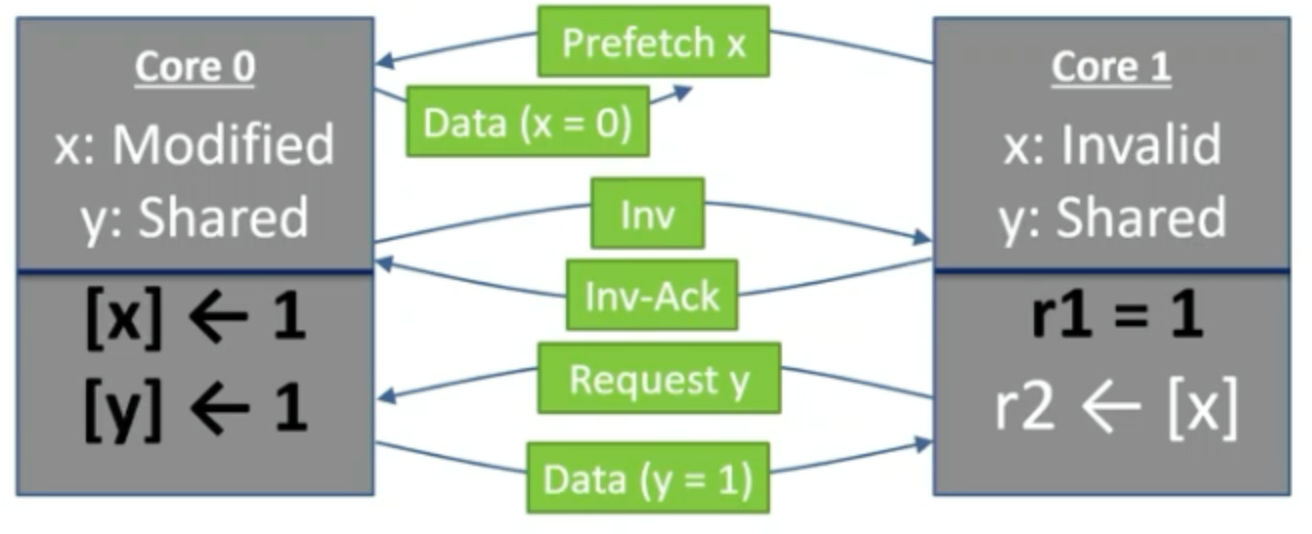
\includegraphics[width=.45\textwidth]{peekaboo.png}}
  \caption{Peekaboo execution trace}
\end{figure}

\subsubsection{Update $\mu$hb (ViCL) for Peekaboo}
Vanilla $\mu$hb graphs do not model per-cache occupancy ($x$ can be 1 in core 1 while being 2 in core 2). Vanilla graphs also do not model the coherence transitions. Value in cache lifetime (ViCL) abstraction augments the graph by providing the missing information.
\medskip\noindent\newline
Each cache line is uniquely identified (in terms of temporal and spatial existence). Each ViCL starts at $\texttt{ViCL}_{create}$ and ends at $\texttt{ViCL}_{expire}$.
\medskip\noindent\newline
Consider the co-mp litmus test (TSO allows $r1=2, r2=2$):

\noindent\begin{minipage}{.2\textwidth}
\captionsetup{labelformat=empty}
\begin{lstlisting}[
    caption=core 1,
    frame=tlrb, 
    basicstyle=\footnotesize
]{Name}
i1 st x, 1;
i2 st x, 2;
\end{lstlisting}
\end{minipage}\hfill
\begin{minipage}{.2\textwidth}
\captionsetup{labelformat=empty}
\begin{lstlisting}[
    caption=core 2,
    frame=tlrb,
    basicstyle=\footnotesize
]{Name}
i3 ld r1, x;
i4 ld r2, x;
\end{lstlisting}
\end{minipage}
\captionof{lstlisting}{Co-mp litmus test}

\noindent\newline
A ViCL timeline would look like the following:
\begin{figure}[H]
  \centering{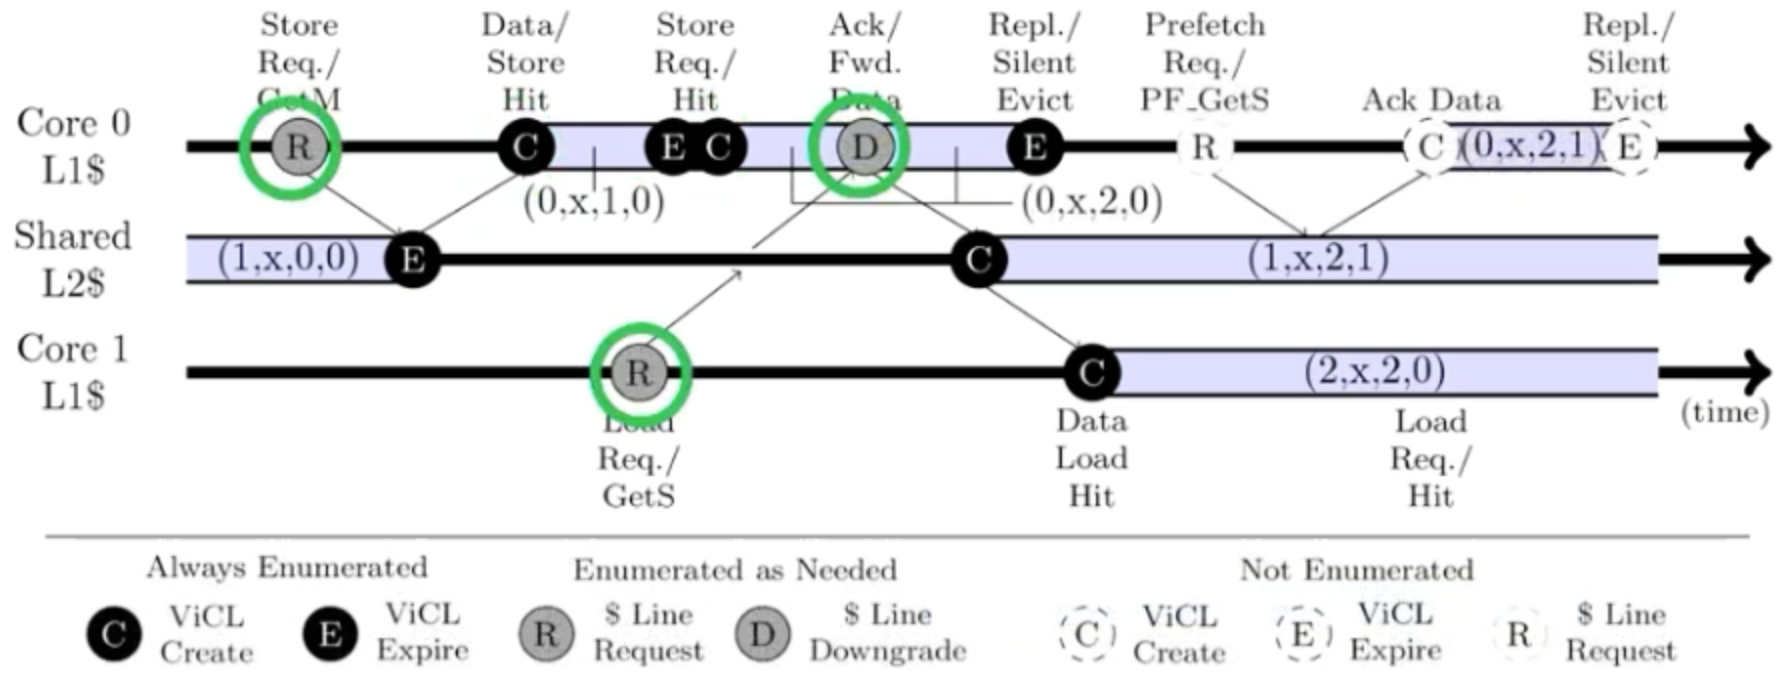
\includegraphics[width=.49\textwidth]{VICL_time.png}}
  \caption{ViCL timeline trace}
\end{figure}

\noindent\newline
With the ViCL augmentation in mind, the new $\mu$hb graph for the MP litmus test would look like the following

\begin{figure}[H]
  \centering{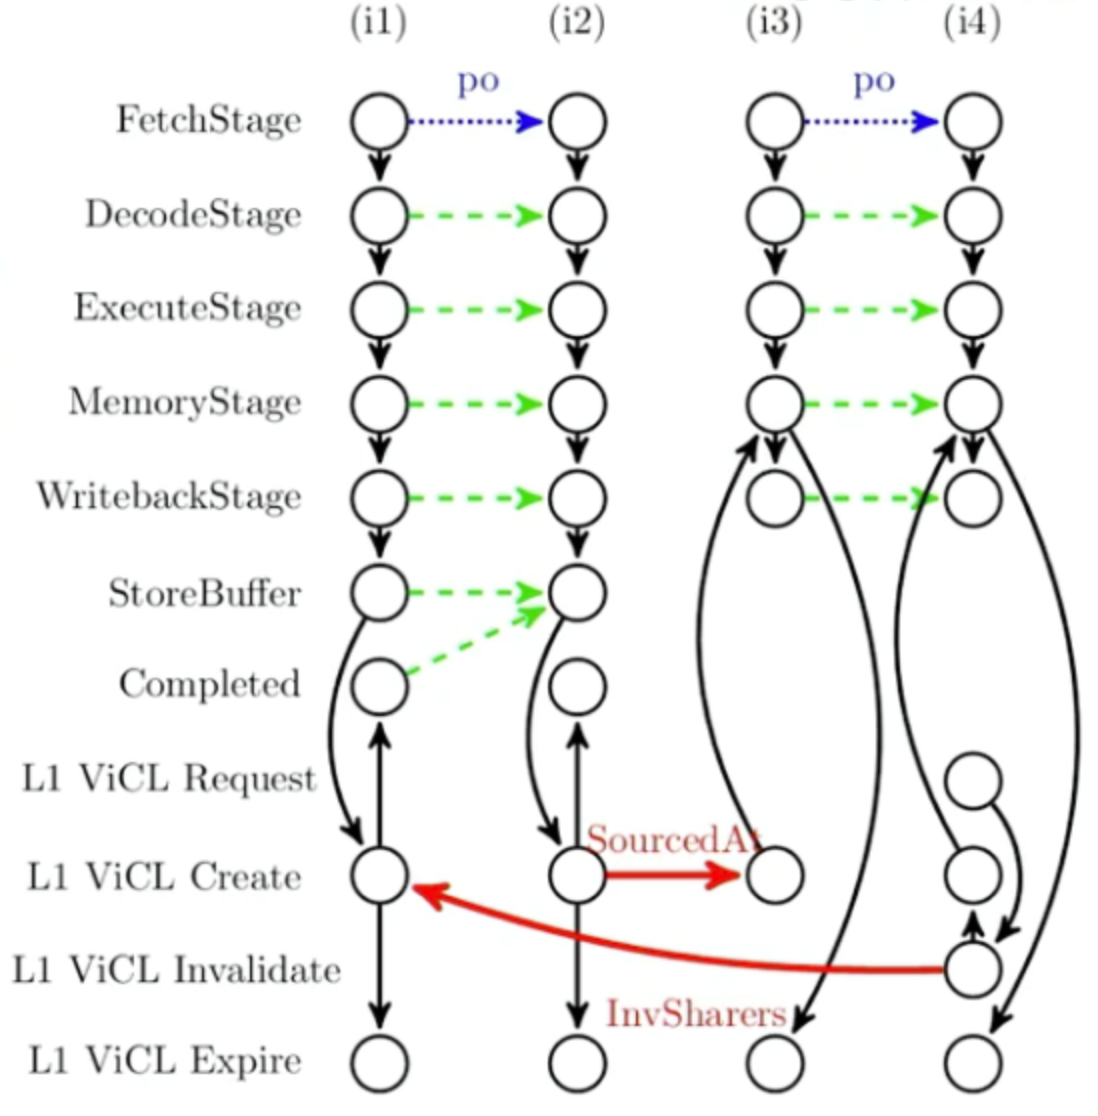
\includegraphics[width=.49\textwidth]{uhb_vicl.png}}
  \caption{Augmented $\mu$hb graph}
\end{figure}

\noindent\newline
Note that the $\texttt{ViCL}_{request}$ is not tied to any node in $i4$, which meant that the prefetch for data can happen ahead of time. Also the ViCL creation in $i4$ is after the invalidation, meaning that the data arrived after the invalidation is processed.

\subsubsection{Solution to the Peekaboo problem}
We can solve the Peekaboo problem by removing one of the optimizations with some caveats in mind. Again from the MP litmus test:
\begin{itemize}
    \item Remove Invalidation before use: Core 1 prefetches y while core 2 prefetches for x. When x is attempting a store to 1 in core 1, core 2 has to perform 1 operation after attempting to read from y (due to TSO ordering) -- hence blocking the store of x. Core 2 requests y from core 1 which is blocked due to store to x has to happen first -- but store to x is blocked. This optimization removal would result in deadlock.
    \item Livelock avoidance: Some core might not be able to load a cache line due to other cores constantly storing to it -- resulting in livelock.
    \item Prefetching: All memory requests are issued in order -- which impacts performance.
\end{itemize}

\noindent\newline
The Peekaboo instruction (load of x) has to be the oldest load/store in program order in order to avoid the Peekaboo problem. Considering the co-mp litmus test, the prior memory operation ($i3$) has to happen before the request is issued (added Peekaboo solution edge). A cycle is detected -- hence not observable -- when adding the Peekaboo edge to the graph. Refer to section 12.6.1 on how the graph is formulated.

\begin{figure}[H]
  \centering{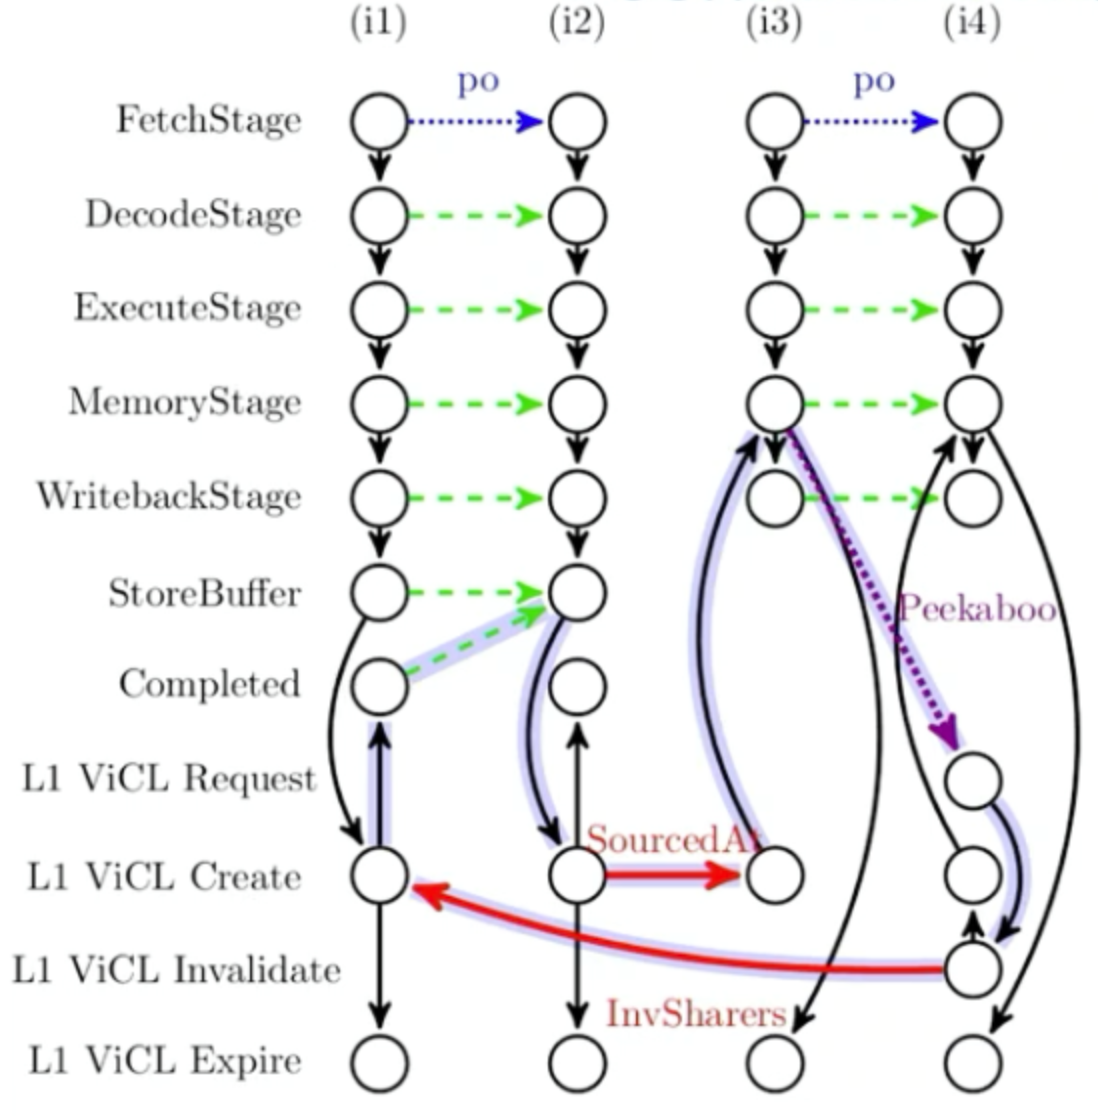
\includegraphics[width=.49\textwidth]{uhb_peekaboo_sol.png}}
  \caption{Augmented $\mu$hb graph}
\end{figure}

\subsection{Lazy Coherence}
Lazy coherence is in the context of having private L1s and shared L2s. The key idea is to enforce coherence at synchronization points (acquires/releases). All prior writes are flushed into the L2 upon a release and all shared lines are self-invalidated upon acquire.

\noindent\begin{minipage}{.2\textwidth}
\captionsetup{labelformat=empty}
\begin{lstlisting}[
    caption=core 1,
    frame=tlrb, 
    basicstyle=\footnotesize
]{Name}
    st 1, x;
rel st 1, y;
\end{lstlisting}
\end{minipage}\hfill
\begin{minipage}{.2\textwidth}
\captionsetup{labelformat=empty}
\begin{lstlisting}[
    caption=core 2,
    frame=tlrb,
    basicstyle=\footnotesize
]{Name}
acq ld r1, y;
    ld r2, x;
\end{lstlisting}
\end{minipage}
\captionof{lstlisting}{Message Passing litmus test}

\noindent\newline
The store 1 to x is flushed to the L2 when executing the release and the acquire would self invalidate (invalid $x, y = 0$) then read the value of y. It is valid for $r1=0; r2=1$ and if we spin on $y$ then we can get $r1=1; r2=1$, which are both valid in SC. If the annotated program is DRF, the lazy coherence is not visible to the programmer.

\noindent\newline
If the program is not annotated, the update to x is possibly not present in the memory hierarchy (L2) could result in $x=0$ due to coherence. An unintuitive outcome of MP would result. Even if the release is present for the store to y, core 2 might have x in its cache and it would not read the updated value in L2.

\noindent\newline
Since lazy coherence only self-invalidate on acquires; no invalidations are sent "out" which reduces false sharing and traffic.

\noindent\newline
In strong MCMs (e.g., TSO), every store is an implicit release and load is an implicit acquire. Lazy coherence in this case would hugely impact performance.

\subsection{Out of Thin Air Values}
Hardware speculation of stores in hardware is generally not a good idea. Usually speculation is not visible to other cores; otherwise, OOTA could result. Also speculation should not break dependencies (i.e., if $i2$ is dependent on $i1$, hardware should not speculate $i2$).

\noindent\begin{minipage}{.2\textwidth}
\captionsetup{labelformat=empty}
\begin{lstlisting}[
    caption=core 1,
    frame=tlrb, 
    basicstyle=\footnotesize
]{Name}
i1 r1 = x;
i2 y  = r1;
\end{lstlisting}
\end{minipage}\hfill
\begin{minipage}{.2\textwidth}
\captionsetup{labelformat=empty}
\begin{lstlisting}[
    caption=core 2,
    frame=tlrb,
    basicstyle=\footnotesize
]{Name}
i3 r2 = y;
i4 x  = r2;
\end{lstlisting}
\end{minipage}
\captionof{lstlisting}{Speculation and OOTA}

\noindent\newline
Speculative store in $i2$ (e.g., 42) visible to all cores might result in OOTA. Core 2 would see the speculation and store it in $r2$, which is then passed to $i4$. $i1$ then loads the value and verified its speculation against itself.

\subsubsection{OOTA due to SW/Compilers}
Consider the following case:

\begin{lstlisting}[
    caption=Compiler Optimizations and OOTA,
    language=C++,
    frame=tlrb,
    basicstyle=\footnotesize
]{Name}
// i is incremented on either branch!
if(x){
    a[i++] = 1;
}
else{
    a[i++] = 2;
}
\end{lstlisting}

The compiler optimization can hoist i out of the if-else statement, but it breaks a load-to-store dependency (i.e., load to $x$ $\rightarrow$ store to $i$).

\subsection{Instruction Dependencies}
Dependencies can be used to enforce local ordering, but it does not state anything about write atomicity. (Dependencies cannot be utilized as fences) There are 3 types of dependencies:

\begin{itemize}
    \item Address dependencies: Result of a load is address for subsequent load or store
    \item Data dependencies: Result of a load is data for a subsequent store
    \item Control dependencies: Result of load controls branch condition, and load or store is after branch in program order
\end{itemize}

\noindent\newline
Not all dependencies have to be enforced. In RISC-V, load-to-load control dependencies are not enforced because it is desired to execute loads after a predicted branch. load-to-store dependencies are enforced since speculative stores are generally a bad idea.

\subsection{Cumulativity}
Consider the following WRC litmus test with local fences (fence that enforces instructions on the same core).

\noindent\begin{minipage}{.15\textwidth}
\captionsetup{labelformat=empty}
\begin{lstlisting}[
    caption=core 1,
    showlines=true,
    frame=tlrb, 
    basicstyle=\footnotesize
]{Name}
x = 1;

 
\end{lstlisting}
\end{minipage}\hfill
\begin{minipage}{.15\textwidth}
\captionsetup{labelformat=empty}
\begin{lstlisting}[
    caption=core 2,
    frame=tlrb,
    basicstyle=\footnotesize
]{Name}
r1 = x;
LOCFENCE;
y  = 1;
\end{lstlisting}
\end{minipage}\hfill
\begin{minipage}{.15\textwidth}
\captionsetup{labelformat=empty}
\begin{lstlisting}[
    caption=core 3,
    frame=tlrb,
    basicstyle=\footnotesize
]{Name}
r2 = y;
LOCFENCE;
r3 = x;
\end{lstlisting}
\end{minipage}
\captionof{lstlisting}{WRC Litmus test}

\noindent\newline
In a MCA/rMCA system, local fences would forbid the non-intuitive outcome of WRC ($r1=1; r2=1; r3=0$). But in nMCA systems, local fences have to be cumulative, when some instruction in a core sees $r1=x$, it also sees $x=1$.

\subsubsection{Lightweight/Heavyweight Fences}
Writes observed before the fence (including writes from other cores) are ordered before writes after the fence using Lightweight fences. However, Lightweight fences do not order writes to subsequent reads, and the forbidden outcome in IRIW ($r1=1; r2=0; r3=1; r4=0$) would be observable. 
\medskip\noindent\newline
For heavyweight fences, all writes observed by the fencing core before the fence must be made visible to all other cores, and all reads before the fence must be performed before any memory operations after the fence are performed -- which forbids unintuitive IRIW.

\noindent\begin{minipage}{.11\textwidth}
\captionsetup{labelformat=empty}
\begin{lstlisting}[
    caption=core 1,
    showlines=true,
    frame=tlrb,
    basicstyle=\footnotesize
]{Name}
A = 1;


\end{lstlisting}
\end{minipage}\hfill
\begin{minipage}{.11\textwidth}
\captionsetup{labelformat=empty}
\begin{lstlisting}[
    caption=core 2,
    frame=tlrb,
    showlines=true,
    basicstyle=\footnotesize
]{Name}
B = 1;


\end{lstlisting}
\end{minipage}\hfill
\begin{minipage}{.11\textwidth}
\captionsetup{labelformat=empty}
\begin{lstlisting}[
    caption=core 3,
    frame=tlrb,
    showlines=true,
    basicstyle=\footnotesize
]{Name}
r1 = A;
lwsync;
r2 = B;
\end{lstlisting}
\end{minipage}\hfill
\begin{minipage}{.11\textwidth}
\captionsetup{labelformat=empty}
\begin{lstlisting}[
    caption=core 4,
    frame=tlrb,
    showlines=true,
    basicstyle=\footnotesize
]{Name}
r3 = B;
lwsync;
r4 = A;
\end{lstlisting}
\end{minipage}
\captionof{lstlisting}{IRIW Litmus test}

\subsection{MCM Formal Verification}

\subsubsection{Instruction-level analysis}
This method would not work for all litmus tests. For TSO with MCA, the following SB litmus test allows $r1=1, r2=0, r3=1, r4=0$. By collating all edges (treating $rf$ the same as $rf_{local}$), a cycle is not equivalent to a forbidden outcome.

\noindent\begin{minipage}{.2\textwidth}
\captionsetup{labelformat=empty}
\begin{lstlisting}[
    caption=core 1,
    frame=tlrb, 
    basicstyle=\footnotesize
]{Name}
i1 x  = 1;
i2 r1 = x;
i3 r2 = y;
\end{lstlisting}
\end{minipage}\hfill
\begin{minipage}{.2\textwidth}
\captionsetup{labelformat=empty}
\begin{lstlisting}[
    caption=core 2,
    frame=tlrb,
    basicstyle=\footnotesize
]{Name}
i4 y  = 1;
i5 r3 = y;
i6 r4 = x;
\end{lstlisting}
\end{minipage}
\captionof{lstlisting}{SB litmus test in TSO}

\begin{figure}[H]
  \centering{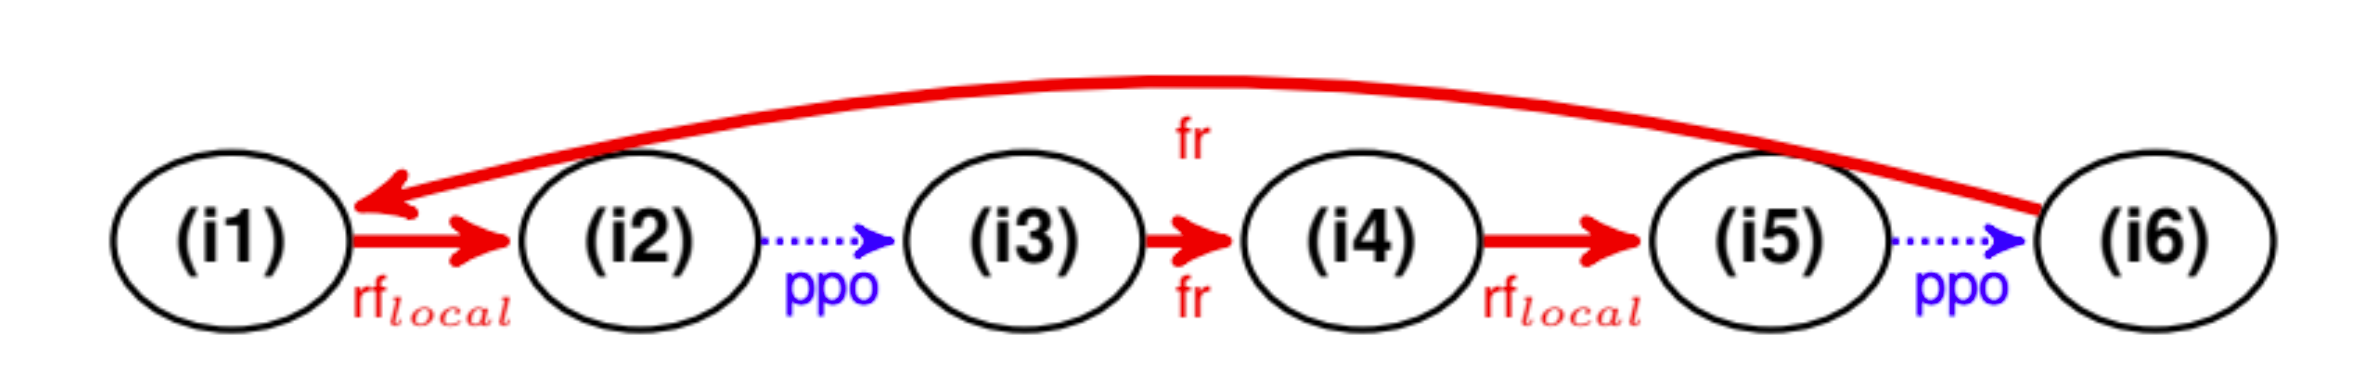
\includegraphics[width=.45\textwidth]{ila_sb.png}}
  \caption{Program analysis of the SB litmus test}
\end{figure}

\subsubsection{$\mu$hb graphs (PipeCheck)}
By including micro-architecture information in happens-before graphs, one could reason whether the micro-architecture is able to generate an observable bug.

\begin{table}[H]
\begin{tabular}{|l|l|l|}
\hline
          & Observable & Unobservable       \\ \hline\hline
Permitted & OK         & OK (HW too strict) \\ \hline
Forbidden & Bug        & OK                 \\ \hline
\end{tabular}
\caption{Analysis and corresponding outcome}
\end{table}

By connecting the nodes specified in the forbidden outcome ($r1=1, r2=0$ for the MP test in TSO), if the graph consists of a cycle, it means that one node has to happen before itself -- which is impossible and deemed not observable.

\noindent\begin{minipage}{.2\textwidth}
\captionsetup{labelformat=empty}
\begin{lstlisting}[
    caption=core 1,
    frame=tlrb, 
    basicstyle=\footnotesize
]{Name}
i1 st 1, x;
i2 st 1, y;
\end{lstlisting}
\end{minipage}\hfill
\begin{minipage}{.2\textwidth}
\captionsetup{labelformat=empty}
\begin{lstlisting}[
    caption=core 2,
    frame=tlrb,
    basicstyle=\footnotesize
]{Name}
i3 ld r1, y;
i4 ld r2, x;
\end{lstlisting}
\end{minipage}
\captionof{lstlisting}{Message Passing Litmus test}

\noindent\newline
By adding required edges to the modeled 5-stage pipeline, we can observe a cycle. If $r1$ has to be 1, the memory stage of $i3$ must happen after update of $i2$ is registered in the memory hierarchy.

\begin{figure}[H]
  \centering{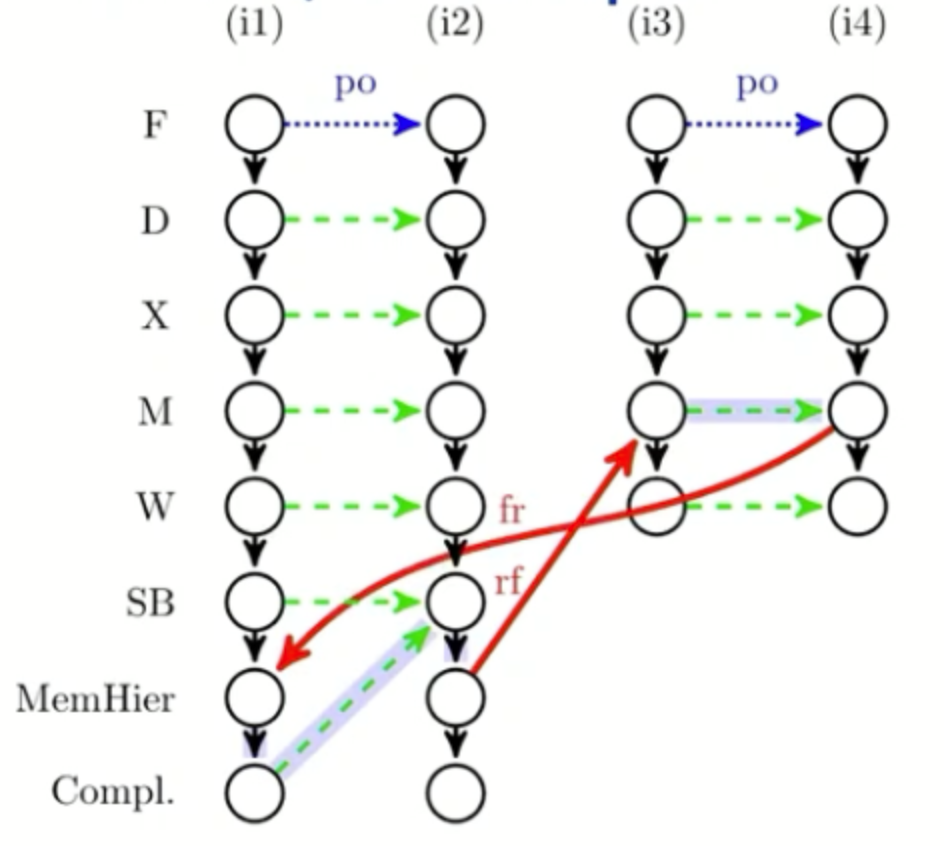
\includegraphics[width=.45\textwidth]{uhb.png}}
  \caption{$\mu$hb graph for 5-stage pipeline}
\end{figure}

\section{Interconnects}
Why having a on chip network (NoCs)? Ad-hoc wiring is not scalable -- area and latency increases for sufficient amount of cores. NoCs are efficient in communication multiplexing and is often modular in nature.

\subsection{Private/Distributed L2}
This section focuses for on shared memory multi-processors where each tile consists of either a distributed or private L2, L1, the core and router. L2s being private though saves bandwidth, might store duplicate data on various tiles. When a miss occurs for a tile with private L2, it contacts the memory hierarchy directly and eventually receives requested data -- total of 2 messages are transmitted. Conversely, in a distributed L2 setup, if a tile contacts another tile for data and a miss occurs, the contacted tile would then contact the memory hierarchy -- total of 4 hops.

\subsection{Coherence and NoCs}
\begin{figure}[H]
  \centering{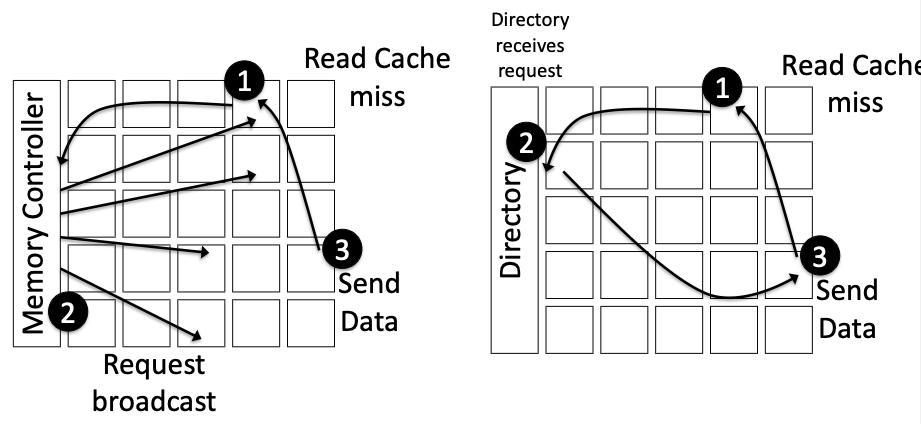
\includegraphics[width=.45\textwidth]{dist_bcast.png}}
  \caption{Broadcast and directories in NoCs}
\end{figure}

\noindent\newline
In directory protocols, since majority requests are unicast, less bandwidth is required for the NoC.

\subsection{NoC switch Topologies}
Out degree is determined by outgoing links from a node and the diameter of a network is the length of the longest of all shortest paths between any two nodes.

\noindent\newline
There are 2 main forms of switch topologies:
\begin{itemize}
    \item Bus: Connects a set of components to a single shared channel -- effective for broadcasting. Buses has a fixed amount of bandwidth.
    \item Crossbar: Directly connects $n$ inputs to $m$ outputs with a single hop.
\end{itemize}

Within switches, there are 2 forms of connectivity:
\begin{itemize}
    \item Direct: All routers are sources and destinations of traffic.
    \item Indirect: Routers are distinct from terminal nodes and intermediate nodes can switch traffic between terminals.
\end{itemize}

There are other several topologies of connecting nodes:
\begin{itemize}
    \item Torus (Direct): $D_n$ dimensional grid with $k$ nodes in each dimension. Denoted as $D_x, D_y, D_z \text{-ary } Num(D) \text{-mesh/cube}$. If end/beginning of rows/columns are connected, it is considered as a cube. Loads in cubed tori are balanced since max path length is $D_n/2$.
    \item Butterfly (Indirect): Each source-destination pair has the same hop count. Traversal is done by looking at the node index bits to select the switch for each stage. An example below shows how node 0 (000) sends a message to node 2 (010). Butterfly networks do not have path diversity -- there is only 1 path for each transmission for given pair of nodes.
    \begin{figure}[H]
        \centering{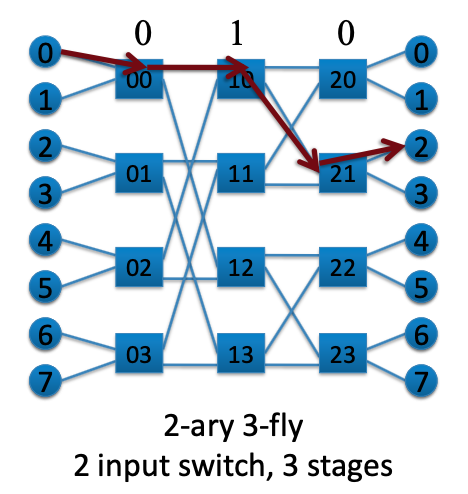
\includegraphics[width=.35\textwidth]{butterfly.png}}
        \caption{Butterfly topology}
    \end{figure}
    \noindent
    By adding an extra layer at the beginning, the first column is free to select any switch in the subsequent layer. Hop count is $Log_kN+1$ and hop count is identical regardless how close 2 nodes are.
    \begin{figure}[H]
        \centering{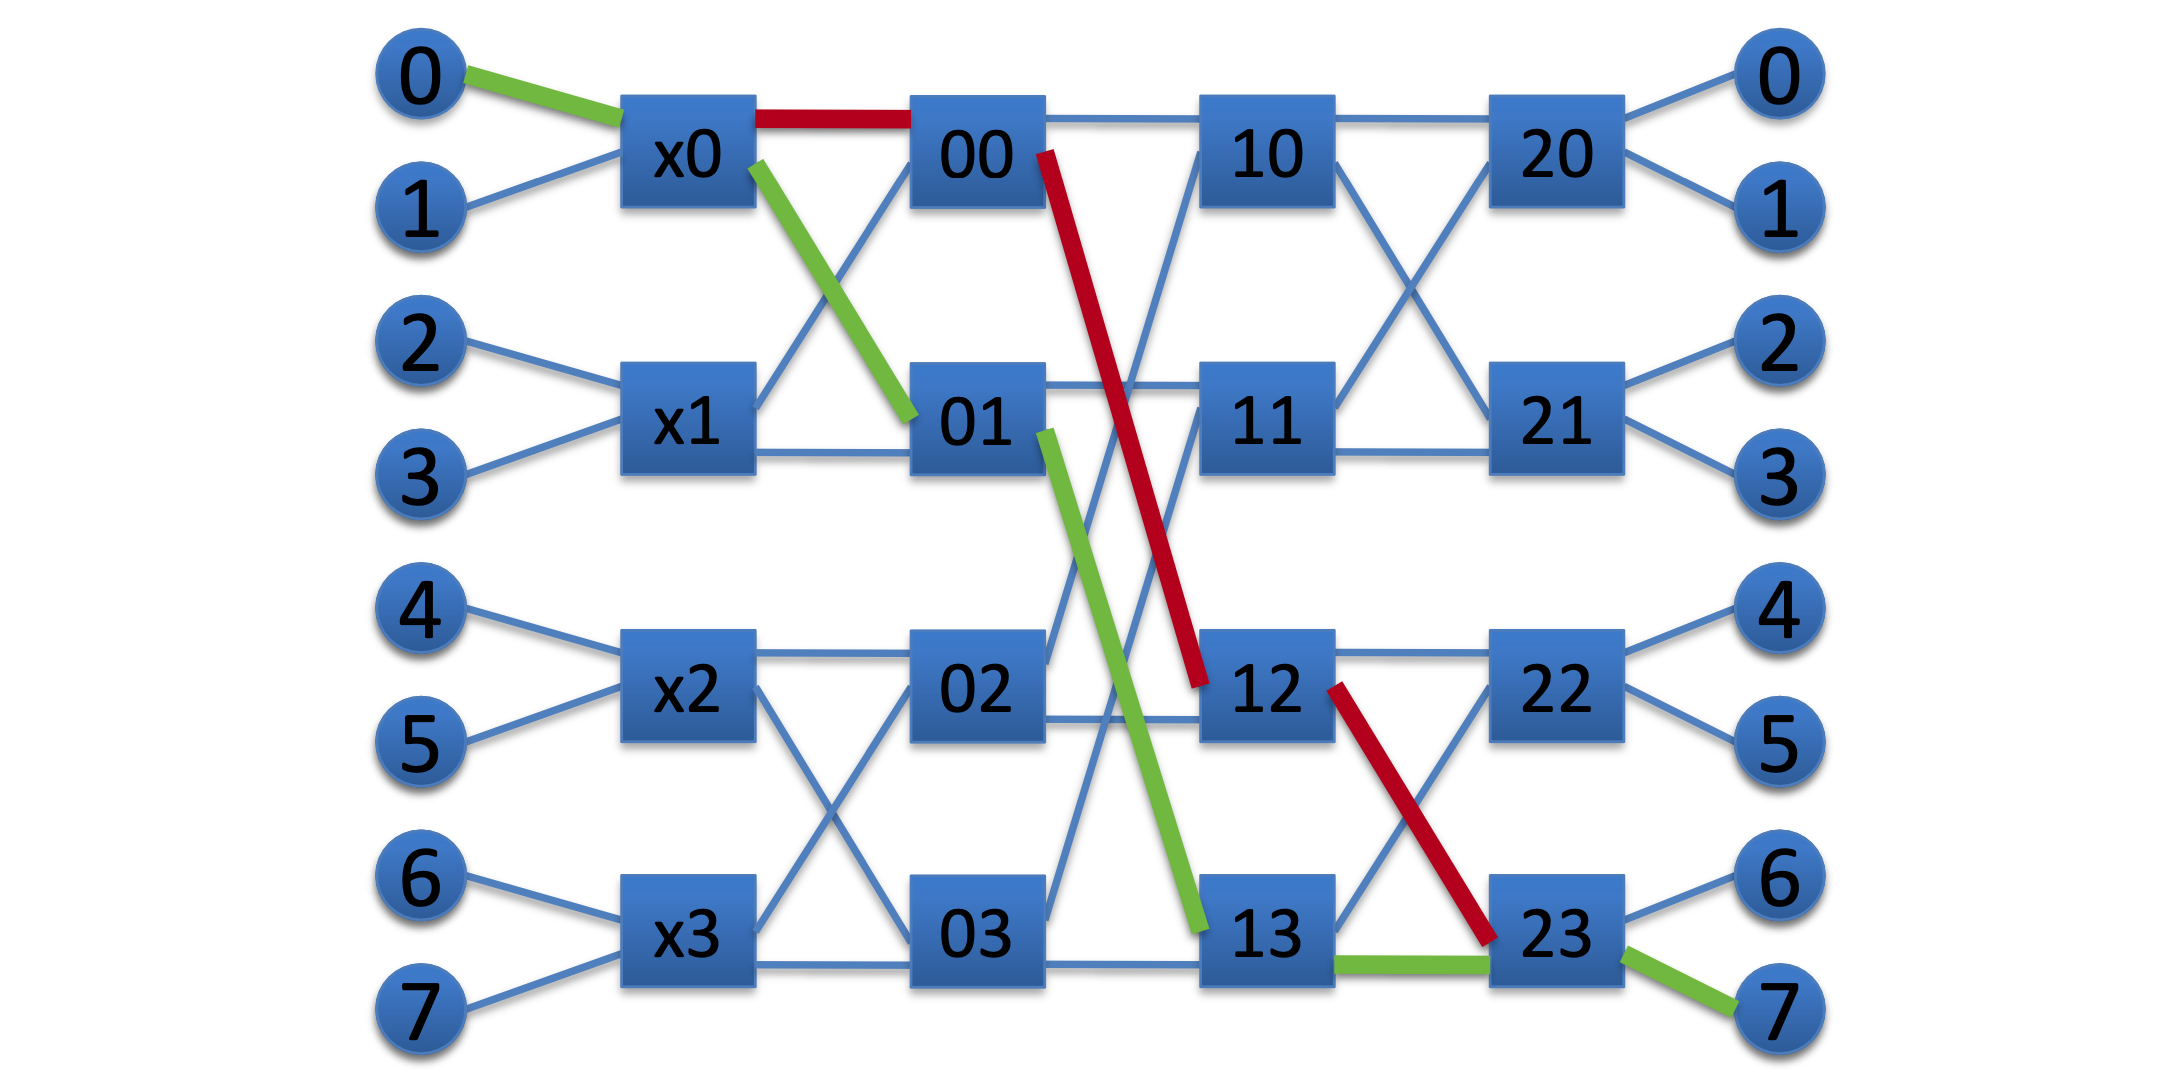
\includegraphics[width=.4\textwidth]{butterfly_extra.png}}
        \caption{Butterfly topology with added layer}
    \end{figure}    
    \item Clos (Indirect): All input/output nodes are connected to all middle routers, meaning that the input is free to choose any middle router which achieves path diversity. The network is parameterized as (middle switches, in/output ports, in/output switches).
    \begin{figure}[H]
        \centering{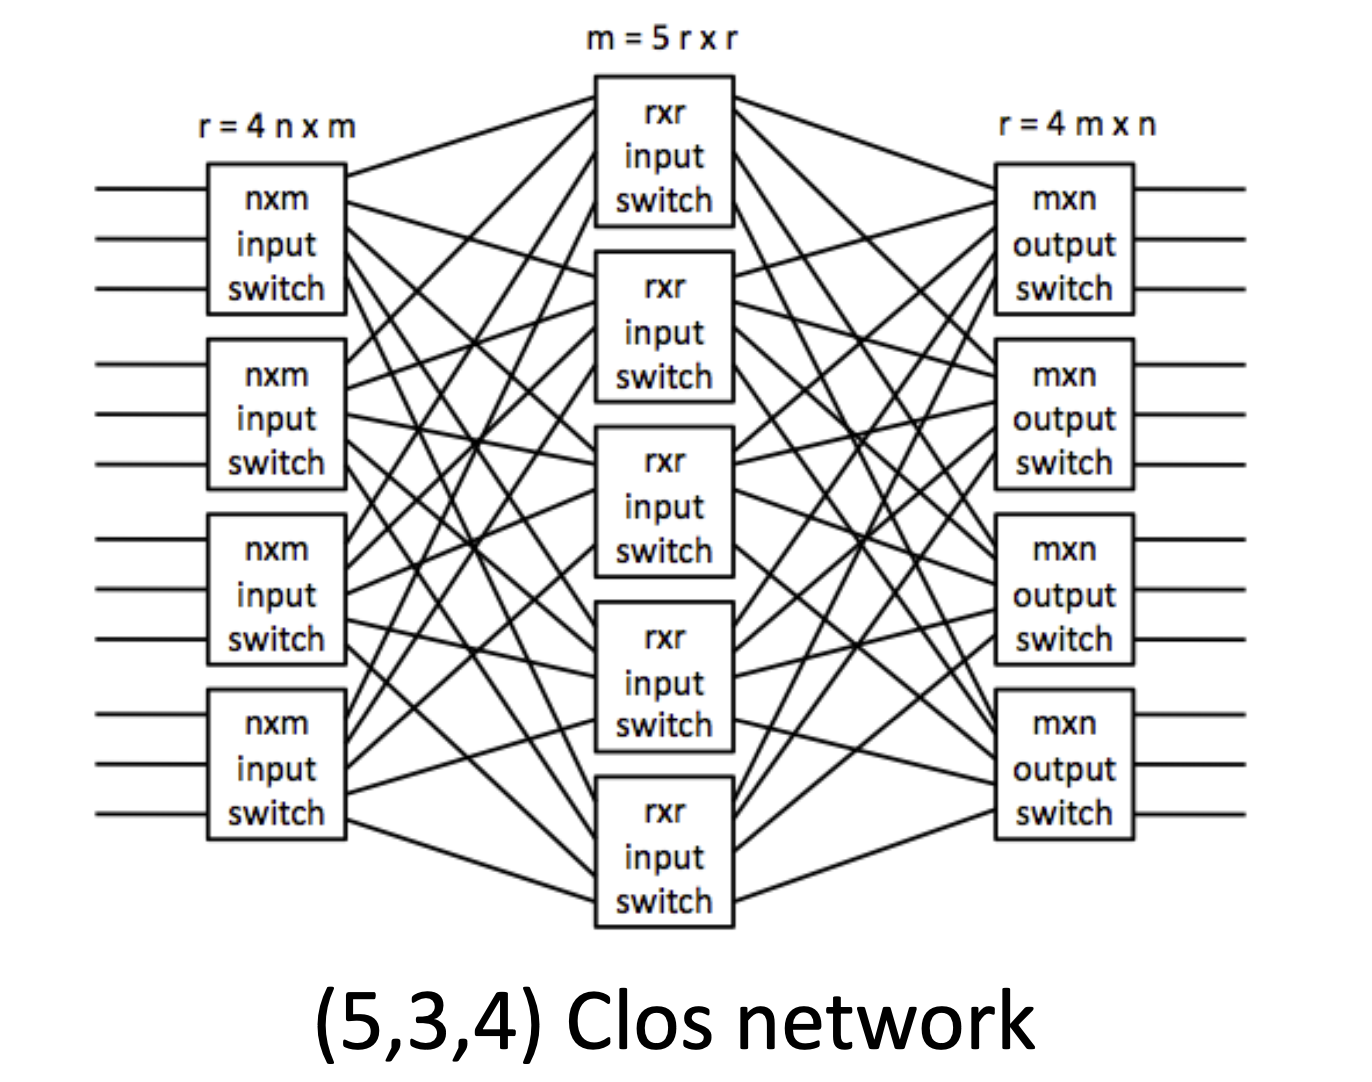
\includegraphics[width=.4\textwidth]{clos.png}}
        \caption{Clos topology}
    \end{figure}      
    \item Fat Tree: Links closer to the root have higher bandwidth. Each node is the leaf of the tree. A message would traverse up to the common ancestor of the source and destination then down to the destination. Fat tree networks can also be designed to be a folded Clos network while pinching the input/output switches.
    \begin{figure}[H]
        \centering{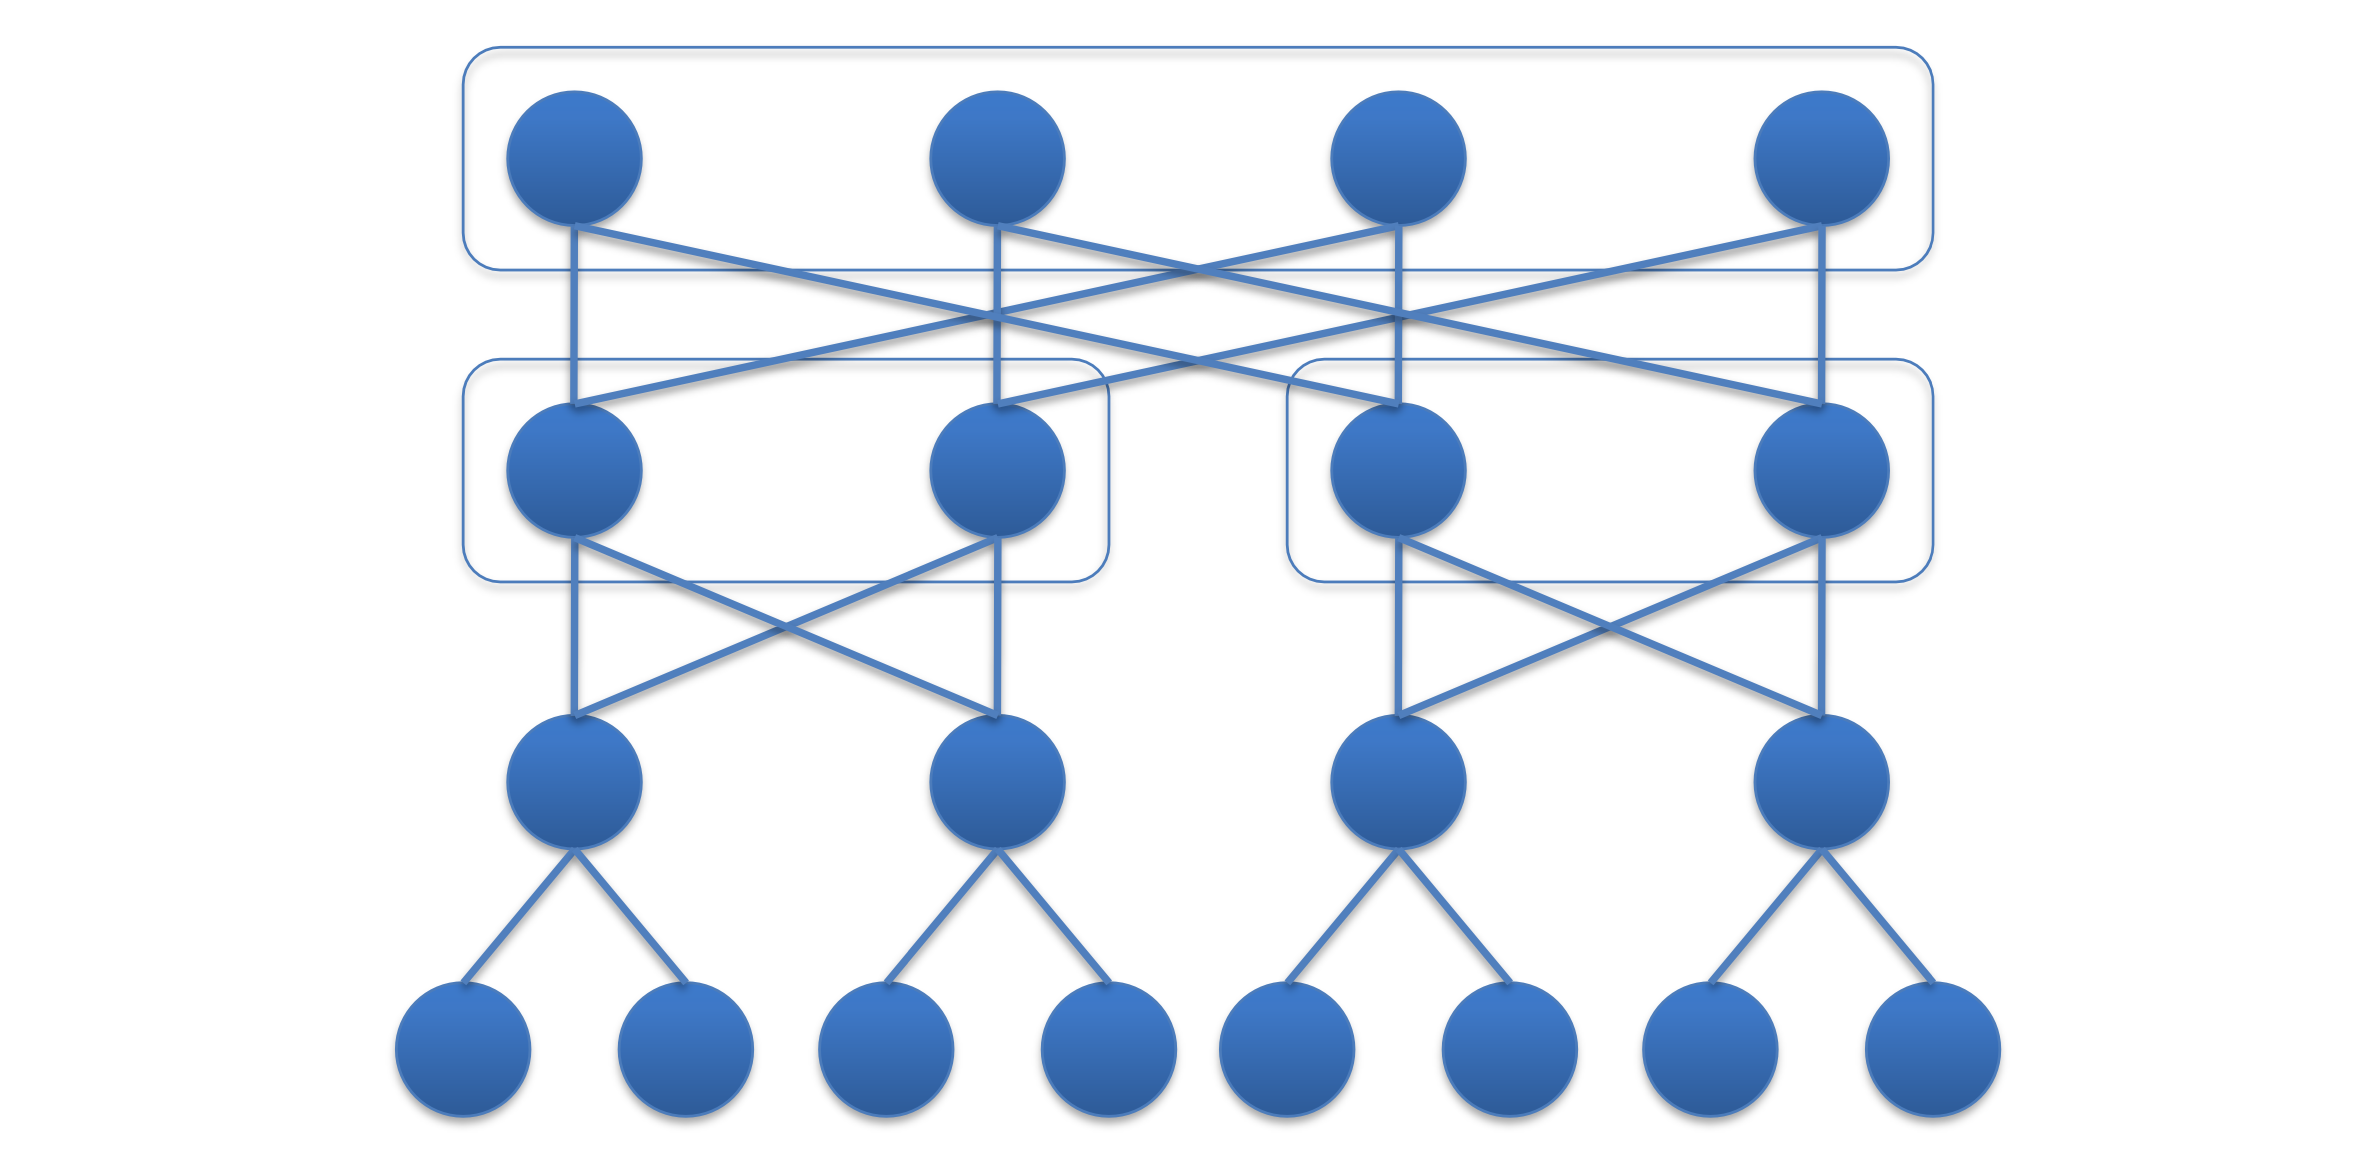
\includegraphics[width=.4\textwidth]{fat_tree.png}}
        \caption{Construct fat tree with Clos}
    \end{figure}      
\end{itemize}

\subsection{Routing in Interconnects}
The goal of routing algorithms is to distribute traffic evenly among paths with reasonable complexity. However, certain routing restrictions are needed to avoid resource contention (deadlock).

\subsubsection{Routing algorithm attributes}
\begin{itemize}
    \item Deterministic: Though simple to implement and deadlock-free, these type of algorithms eliminate path diversity and have poor load balancing.
    \medskip\noindent\newline
    Typical example is the Dimension Order Routing (also called X-Y DOR) which traverse the network in order of dimensions -- only turn to Y after finishing X.
    \item Oblivious: Routing decision are not dependent on network state. An example is the minimal oblivious algorithm where the intermediate nodes lie within the minimum quadrant.
    \item Adaptive: Buffer occupancies are often used to make routing decisions. Global occupancy can be costly to obtain and relying on only local information may lead to sub-optimal results. 
    \medskip\noindent\newline
    Non-minimal (shortest path constraint lifted) adaptive networks allow non-shortest paths but continuous mis-routes may lead to livelock (Circling).
    \medskip\noindent\newline
    The Turn model would forbid some "turns" according to constraints in a specific routing algorithm. If no cycles can happen, then the algorithm is deadlock-free. West-first/North-last/Negative-first constraints are sufficient to guarantee deadlock-free by eliminating 2 edges according to the constraints.
    \begin{figure}[H]
        \centering{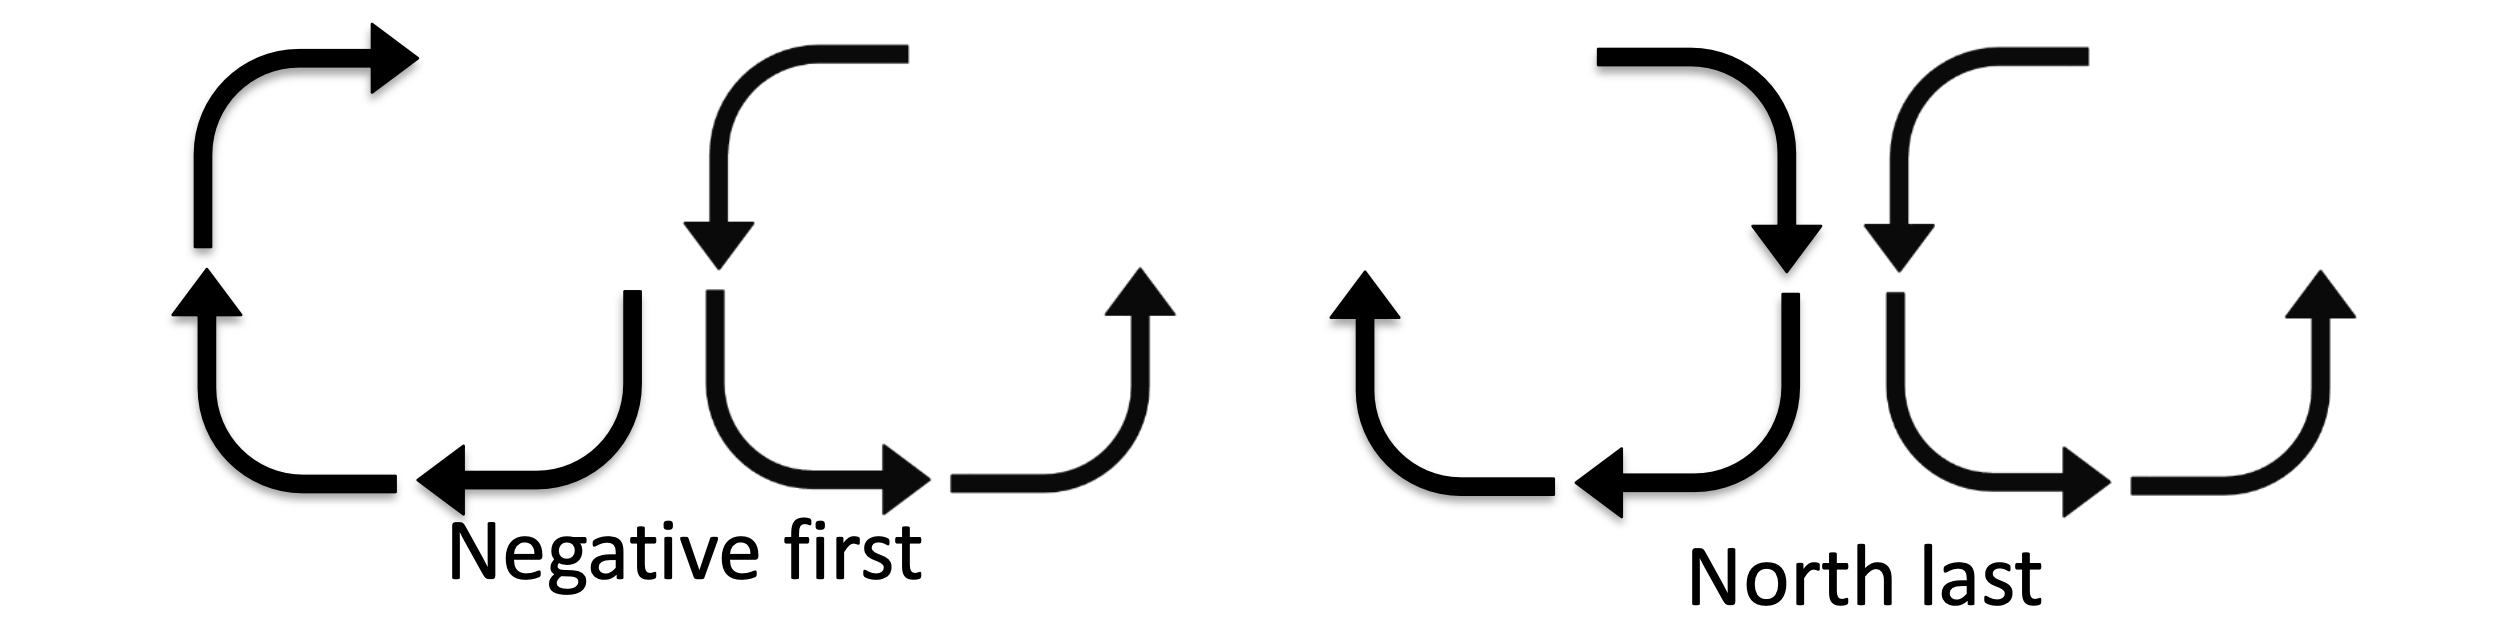
\includegraphics[width=.4\textwidth]{turn_model.png}}
        \caption{Turn elimination that eliminates deadlock}
    \end{figure}        
\end{itemize}

\subsubsection{Routing algorithm implementation}
\begin{itemize}
    \item Source tables: Each node has its own table with specified routes to every node starting from itself; even if the table is reconfigurable, this mechanism cannot adapt to network conditions. This can facilitate lookahead routing to eliminate RC state (See 13.6) at each hop.
    \item Node tables: Instead of storing the entire route, each node only stores the next direction starting from itself.
    \item Combinational circuits: Unlike table-based methods, a circuit has no reconfigurability. Simple algorithms like DOR can be implemented in circuits. The circuit would check how many units the message has to traverse in the x/y direction.
    \begin{figure}[H]
        \centering{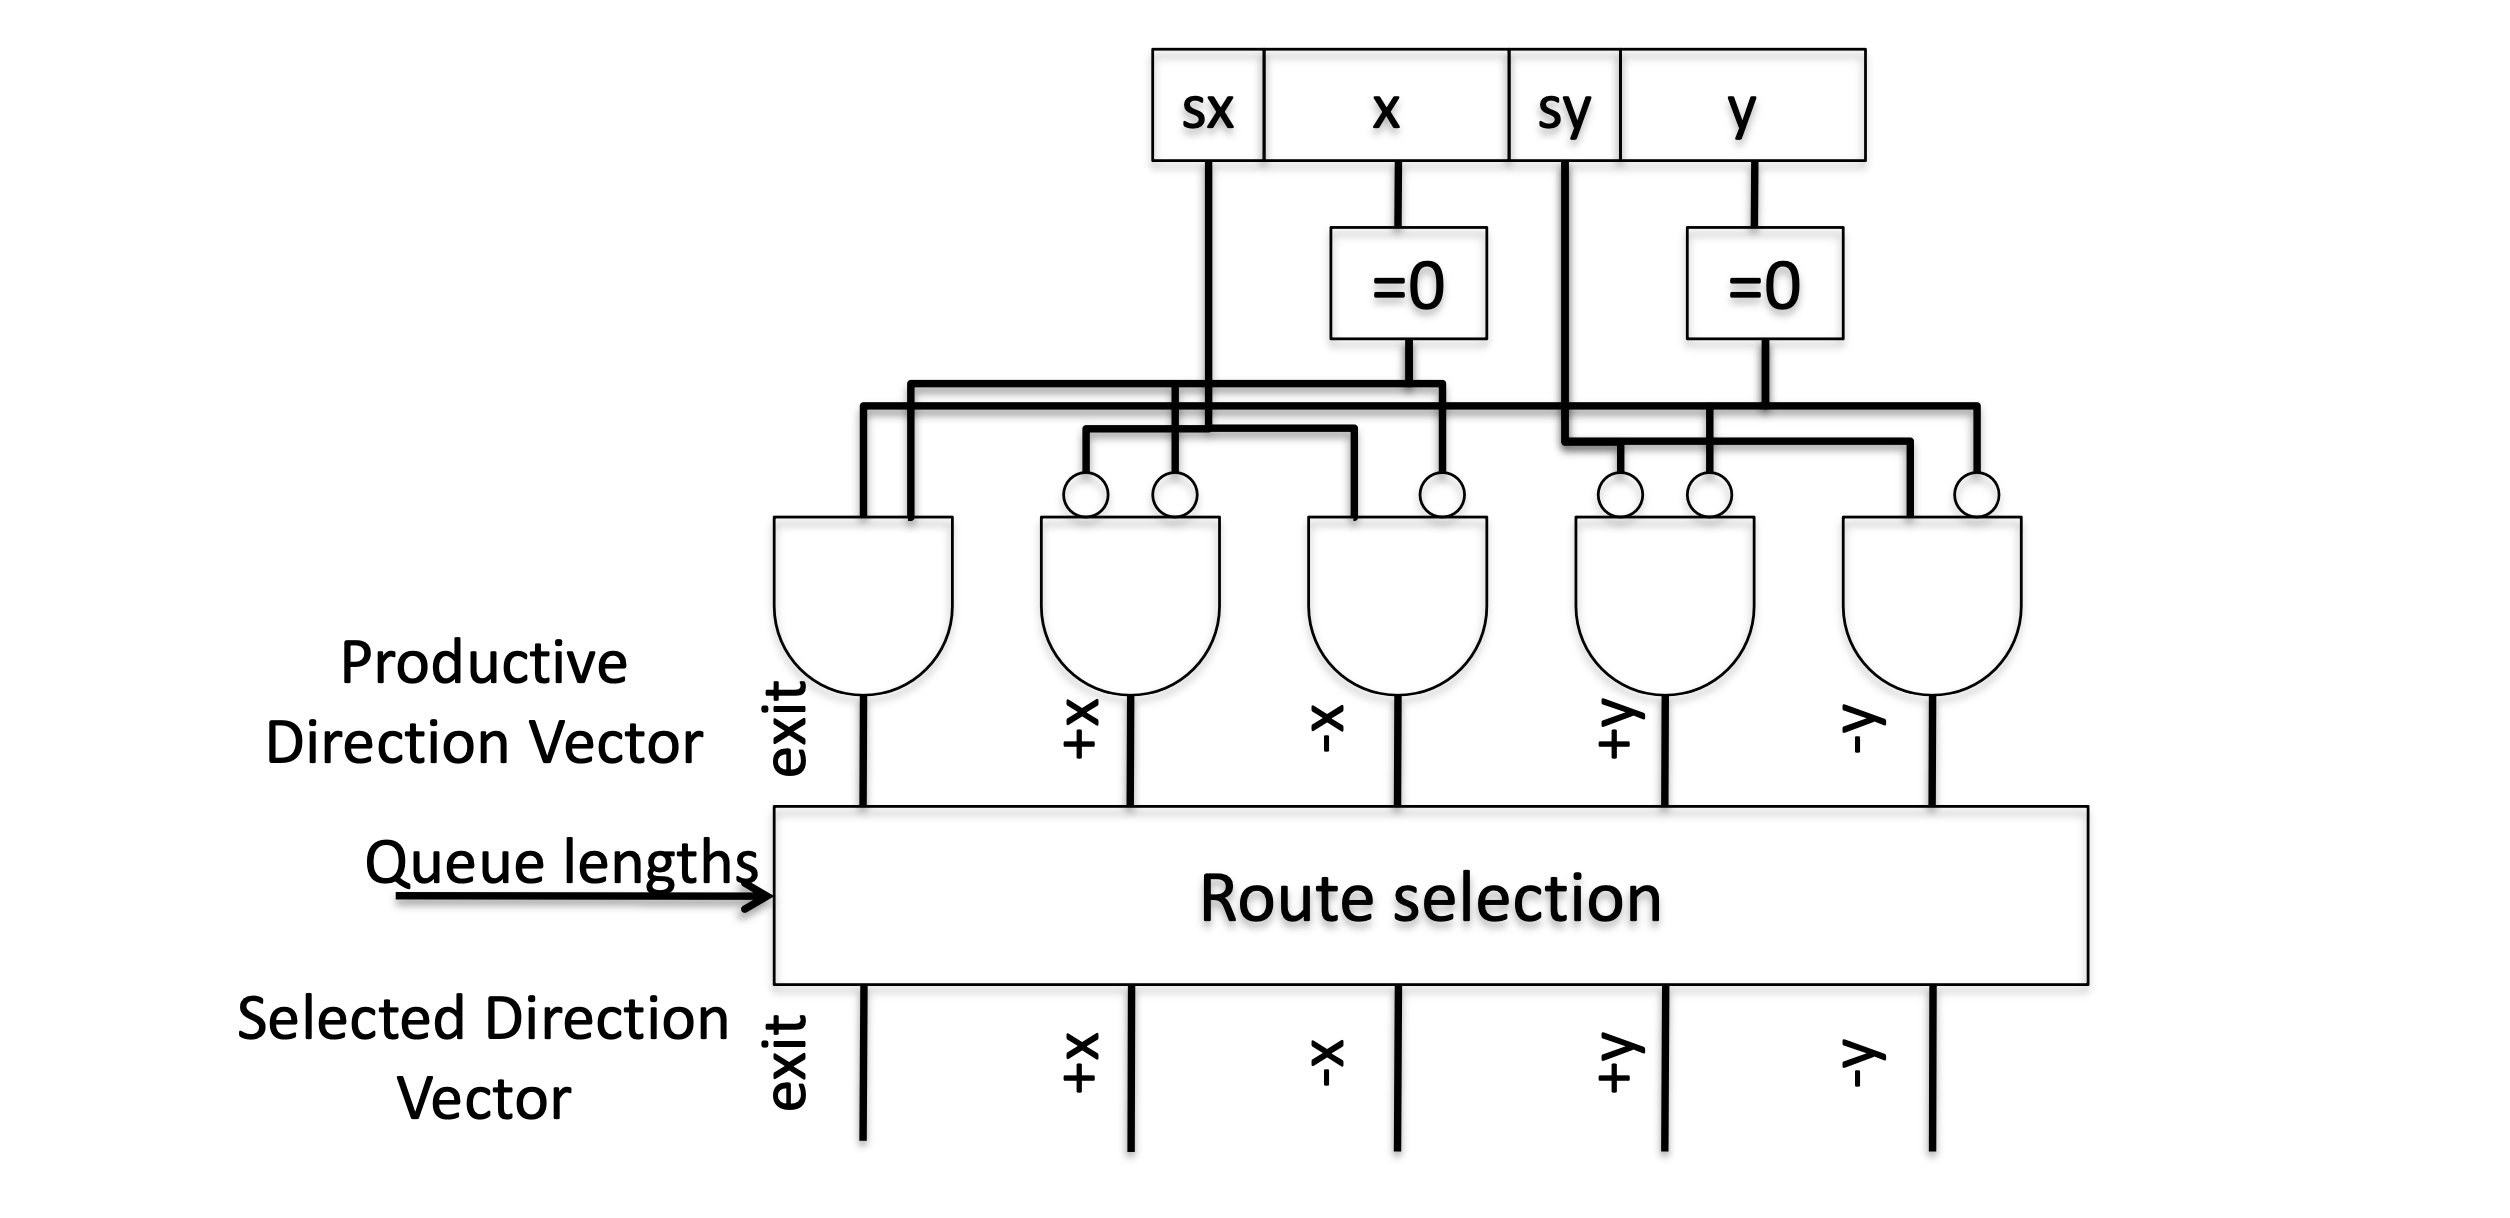
\includegraphics[width=.45\textwidth]{circuit_routing.png}}
        \caption{Circuit based routing algorithm}
    \end{figure}      
\end{itemize}

\subsection{Flow Control in Routing}
Determines allocation of resources to messages as they traverse the network. Control state records the allocation of channels to packets and state of the traversing packet.
\begin{figure}[H]
    \centering{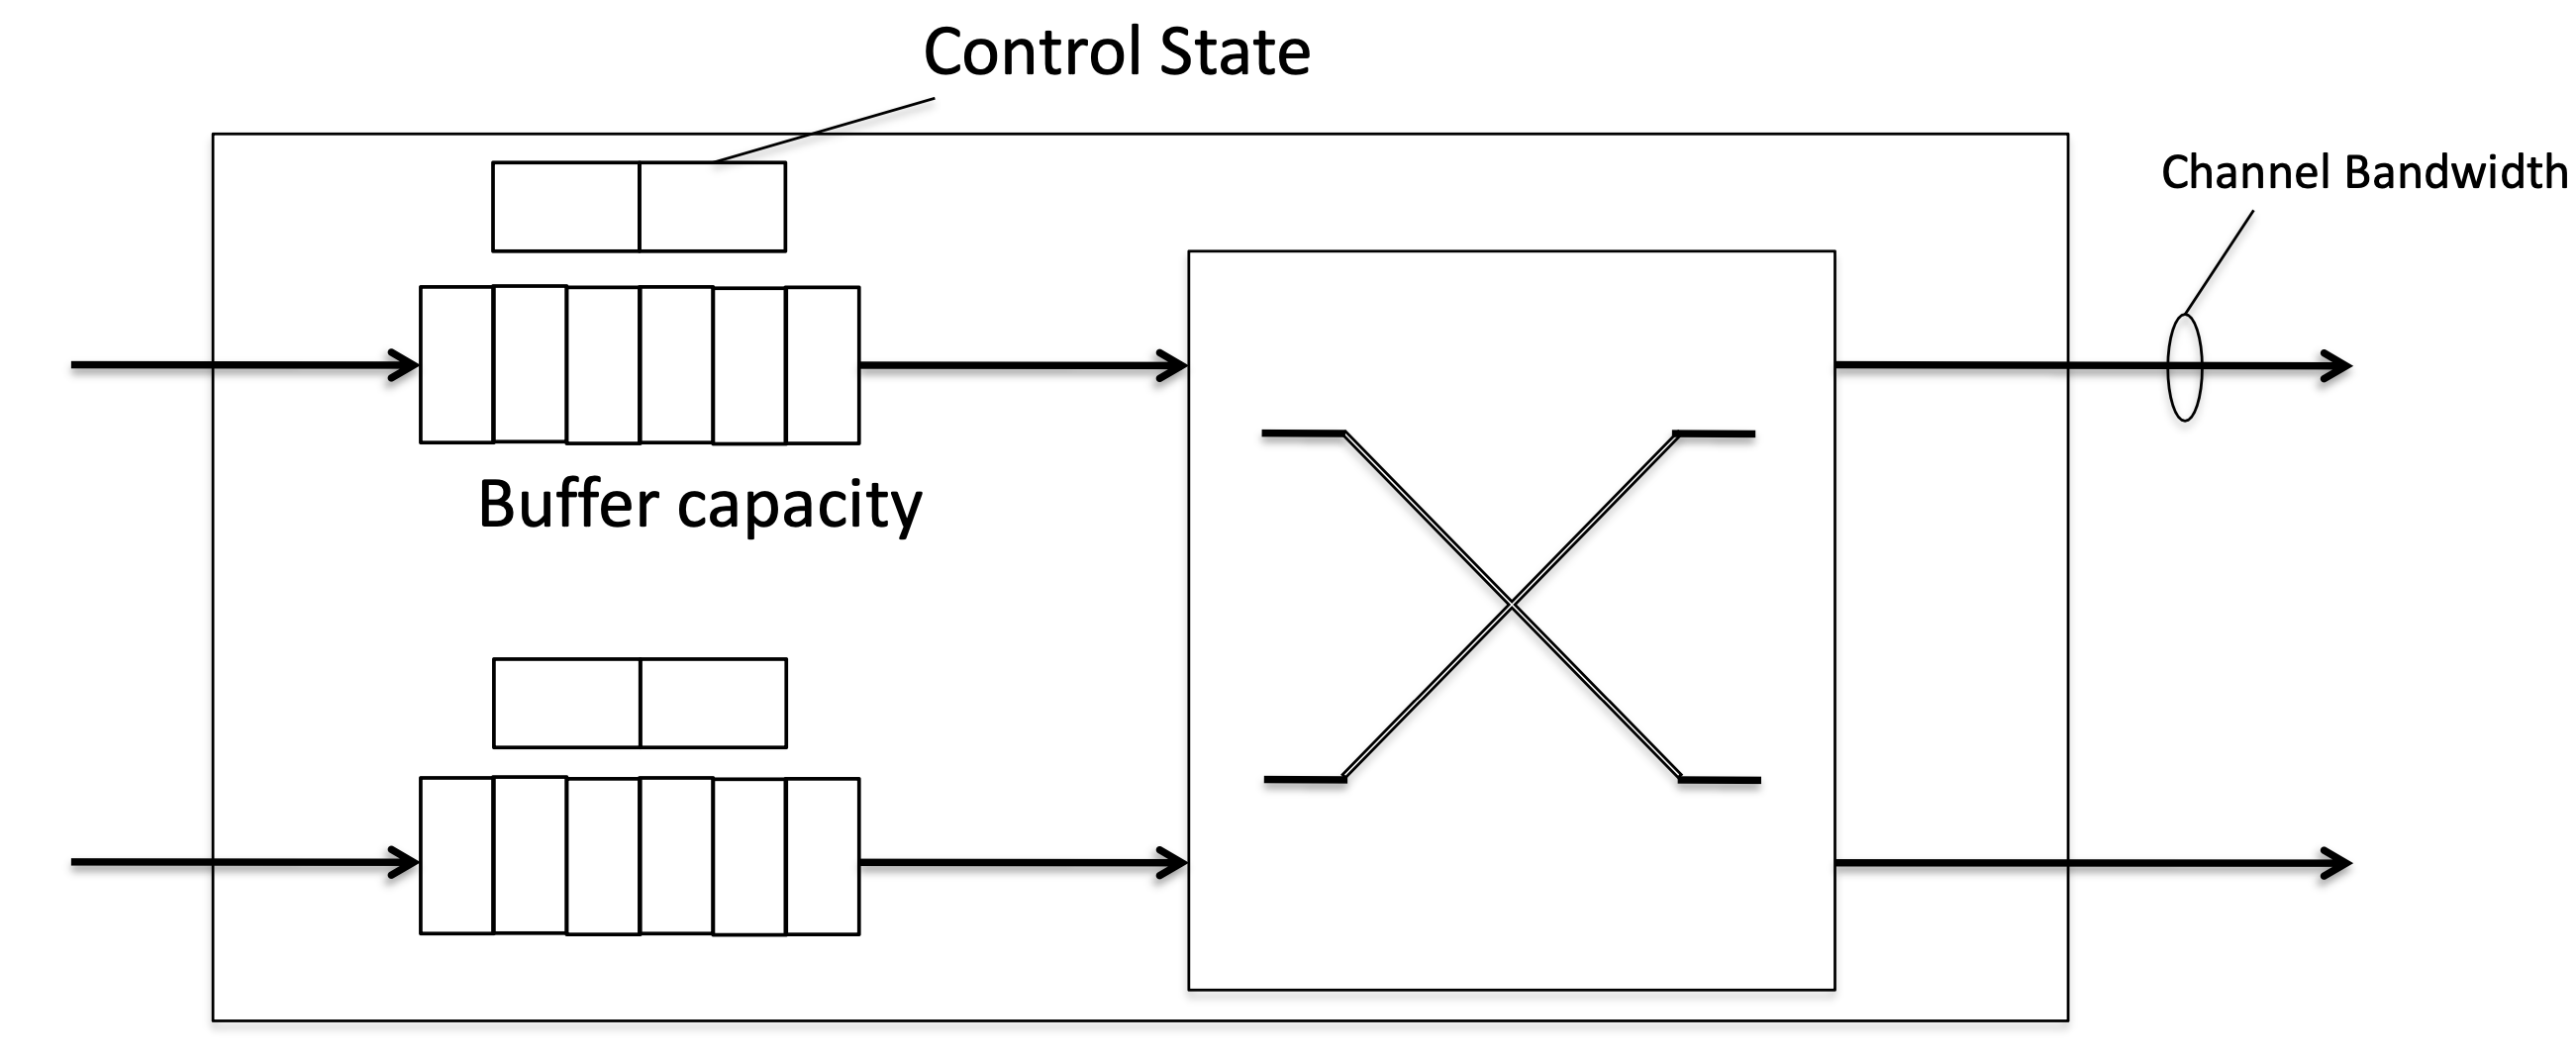
\includegraphics[width=.45\textwidth]{flow_control.png}}
    \caption{Flow control organization}
\end{figure}   
\noindent\newline
Messages are organized by packets and flits. All flits in a packet follow the same route. See below:

\subsubsection{Different types of flow control}
Flow control can be done in various granularity:
\begin{itemize}
    \item Message-based: In \textbf{circuit switching}, it pre-allocates resources across required hops and probes are sent to the network to preserve resources. When a node within the probing path wants to send a request, it has to wait till the preceding circuit switching process is done.
    \begin{figure}[H]
        \centering{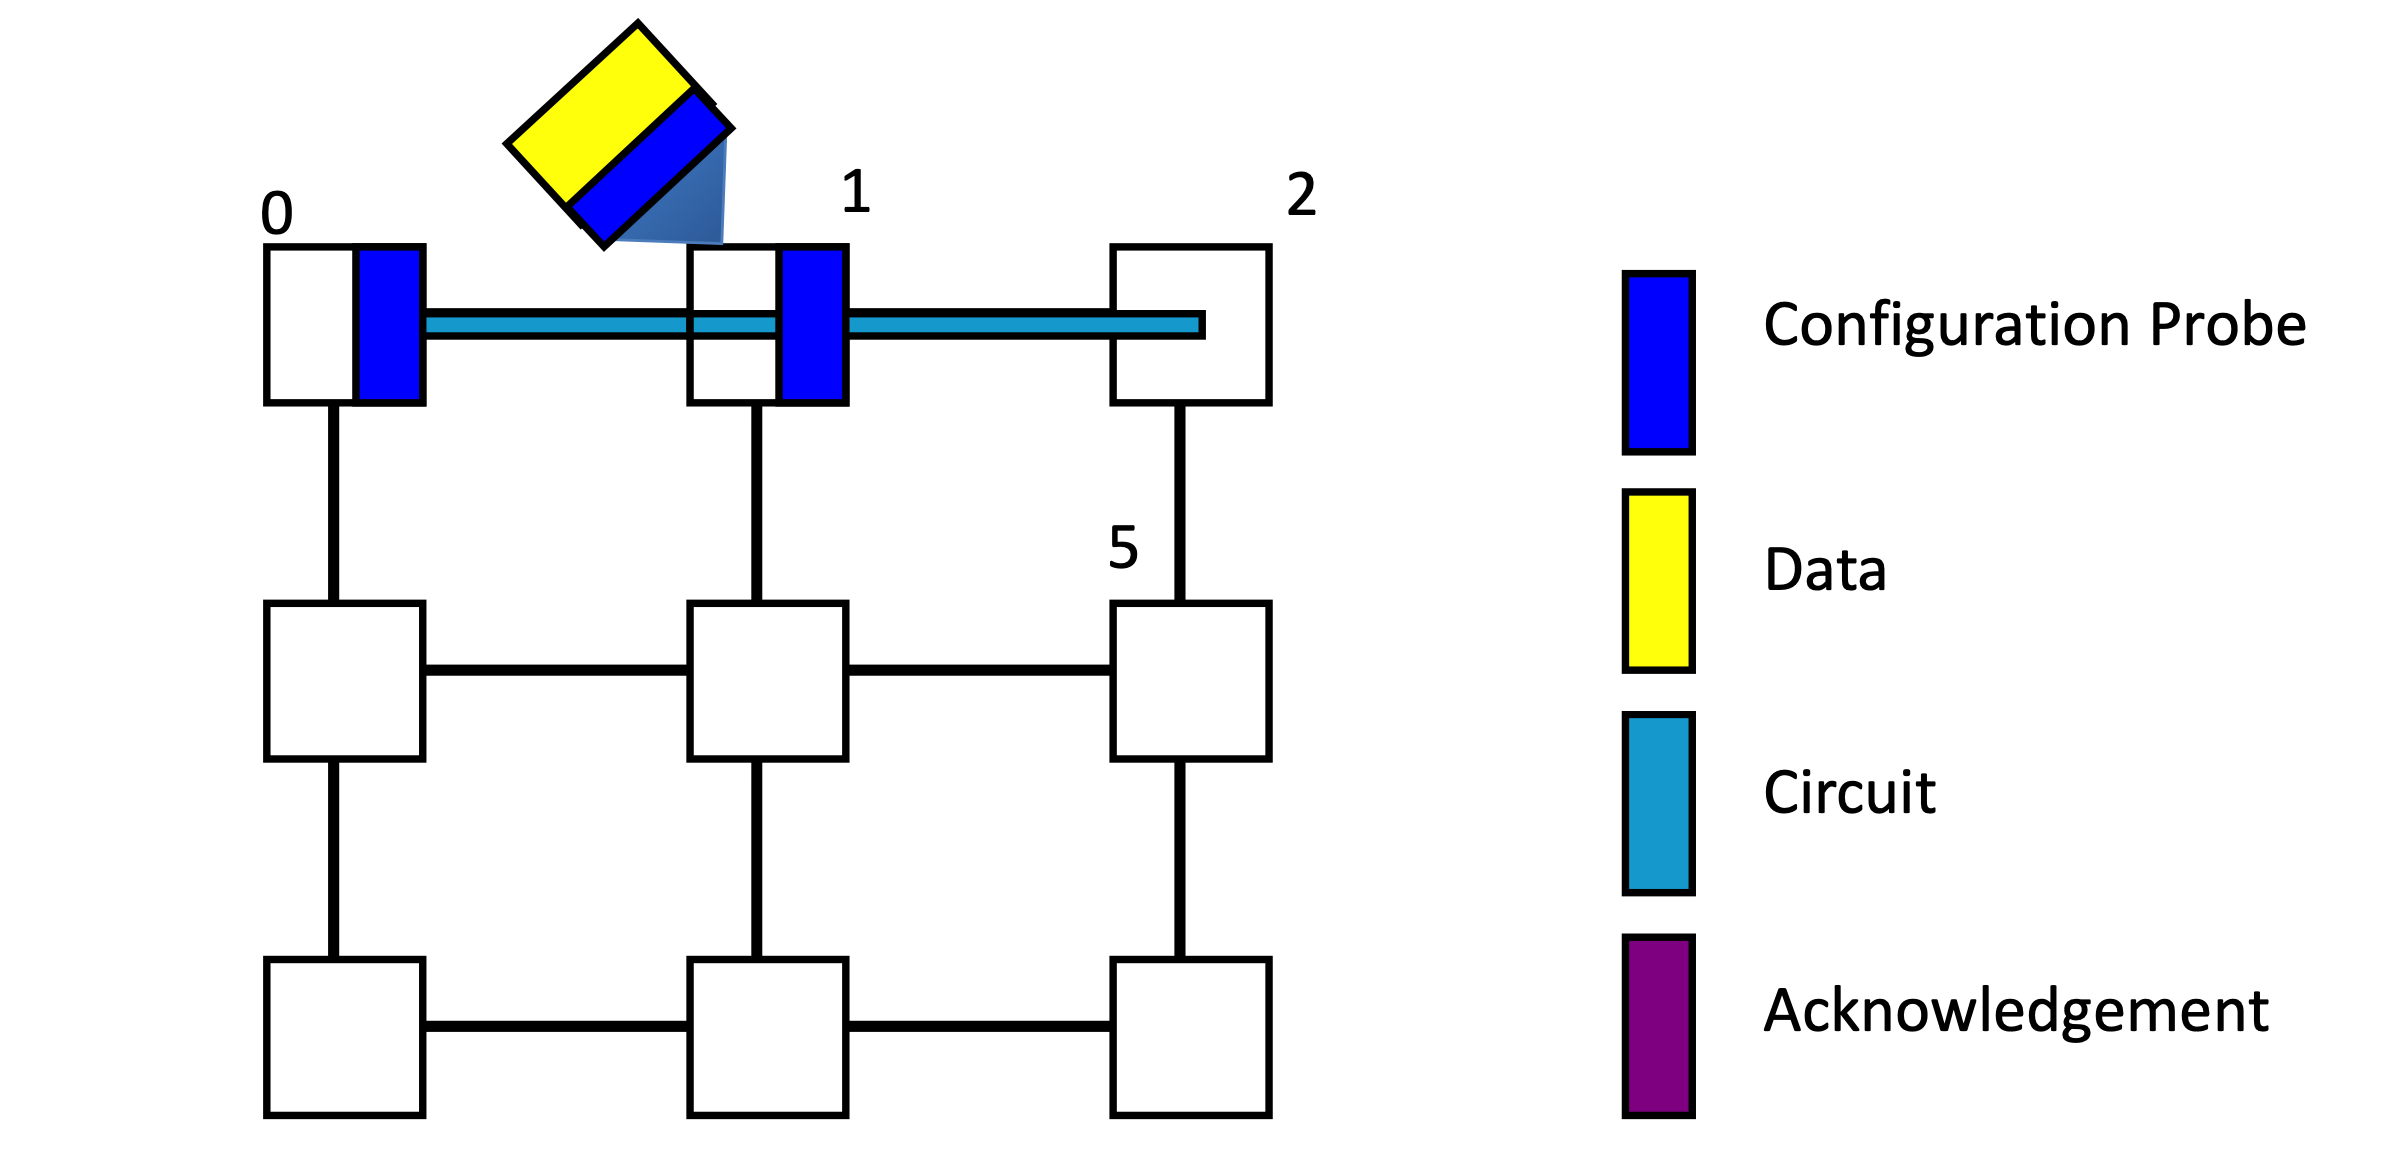
\includegraphics[width=.4\textwidth]{circuit_switching_wait.png}}
        \caption{Contention in circuit switching}
    \end{figure}    
    \item Packet-based: In \textbf{store and forward}, a head flit would wait at the router till the entire packet is received before proceeding to the next hop. In \textbf{virtual cut-through}, flits can proceed without waiting for the tail only if the next router has enough space for the entire packet.
    \item Flit-based: In \textbf{wormhole flow control}, the buffer space in the next router only requires a single flit. However, head flits of some packet can be sent out only when the flits of the preceding packet exits the router.
    \begin{figure}[H]
        \centering{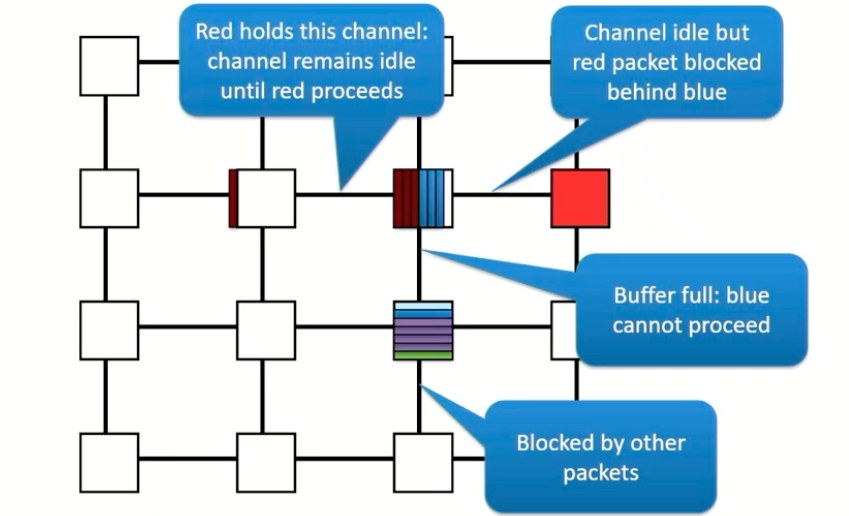
\includegraphics[width=.45\textwidth]{wormhole_wait.png}}
        \caption{HOL blocking in wormhole flow control}
    \end{figure}      
\end{itemize}

\subsubsection{Virtual channels}
Virtual channels are supposedly used to solve head-of-line blocking in wormhole flow control. Consider the case how virtual channels change the timeline for the previous transmission route:
\begin{figure}[H]
    \centering{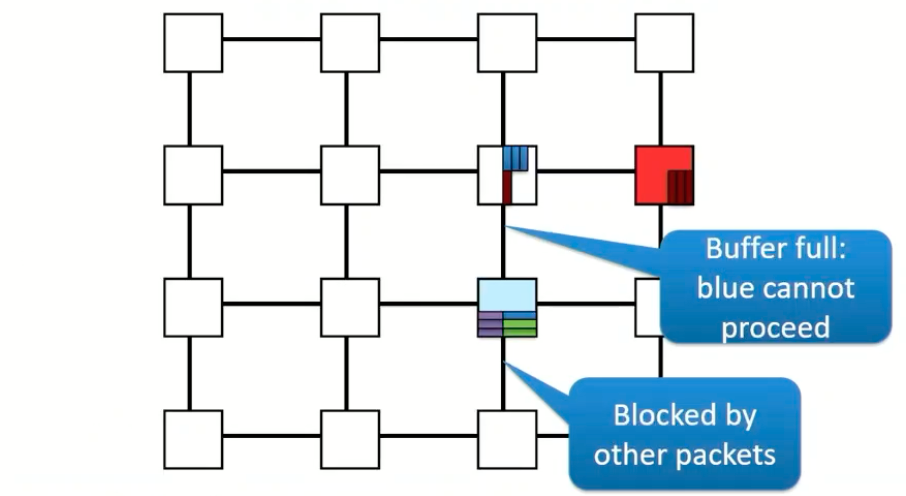
\includegraphics[width=.45\textwidth]{vc_hol.png}}
    \caption{VCs solving HOL}
\end{figure}
\noindent\newline
Links are not idle when upstream is throttling because it might be used by packet allocated to other VCs.
\subsubsection{Deadlock and flow control}
Virtual channels (VC) can break resource cycles if the routing algorithm is not deadlock-free. If lower priority VC cannot request for high priority VCs, thus it breaks possible link cycles. In other words, since deadlock requires for 2 channels to depend each other, not allowing the lower priority VC to request for higher priority VC breaks the dependency.
\medskip\noindent\newline
By enforcing ordering among VCs, this would lower VC utilization since lower priority VCs would only receive data after the dateline. By employing an escape VC (a VC that uses deadlock-free routing like DOR), flits that are stuck can escape to the escape VC would eventually guarantees that the flit would reach its destination.

\subsubsection{Buffer backpressure in routers}
\begin{itemize}
    \item Credit-based: For the upstream router, credit is decremented when forwarding a flit and stops sending with no credit available. When the buffer is freed, the downstream router sends credit to the upstream router. For a single buffer setup, throughput would suffer due to extra credit information being sent out for every forwarded flit.
    \begin{figure}[H]
        \centering{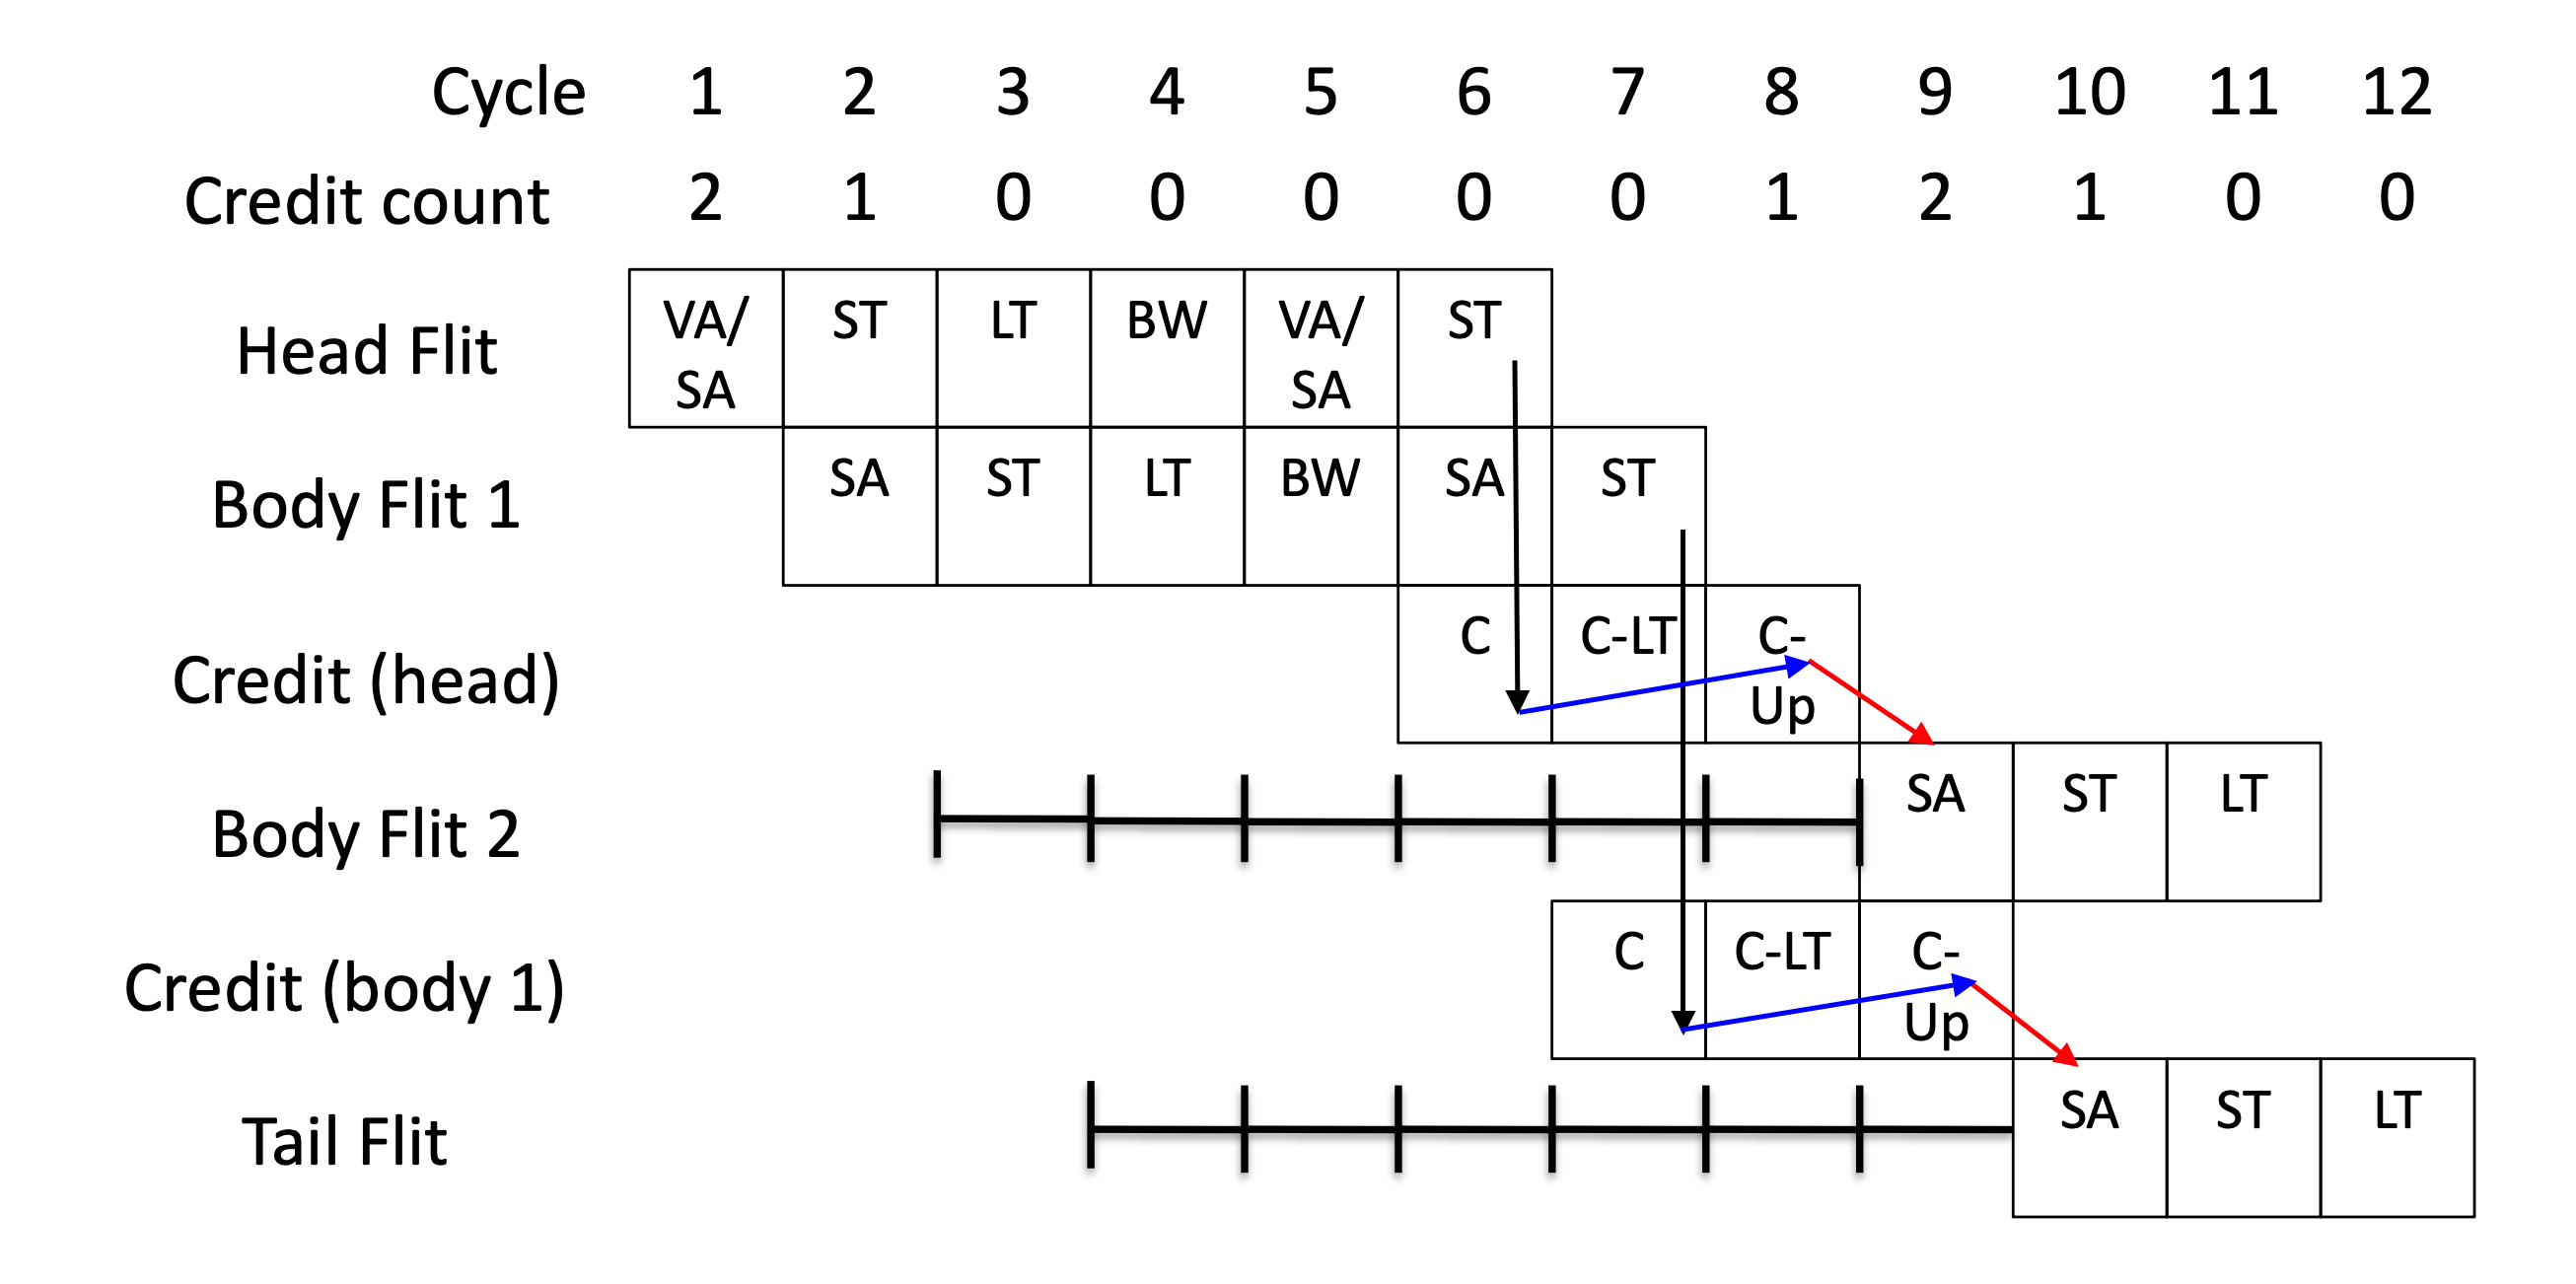
\includegraphics[width=.45\textwidth]{credit.png}}
        \caption{Credit timeline}
    \end{figure}    
    \item On-Off based: Sends an off signal when free buffers are below a threshold and sends an on signal when free buffers are above a threshold. But $Sig_{off}$ needs to be set early enough to prevent buffer overflowing, while $Sig_{on}$ needs to be sent early enough before the buffer is empty and has nothing to send.
    \begin{figure}[H]
        \centering{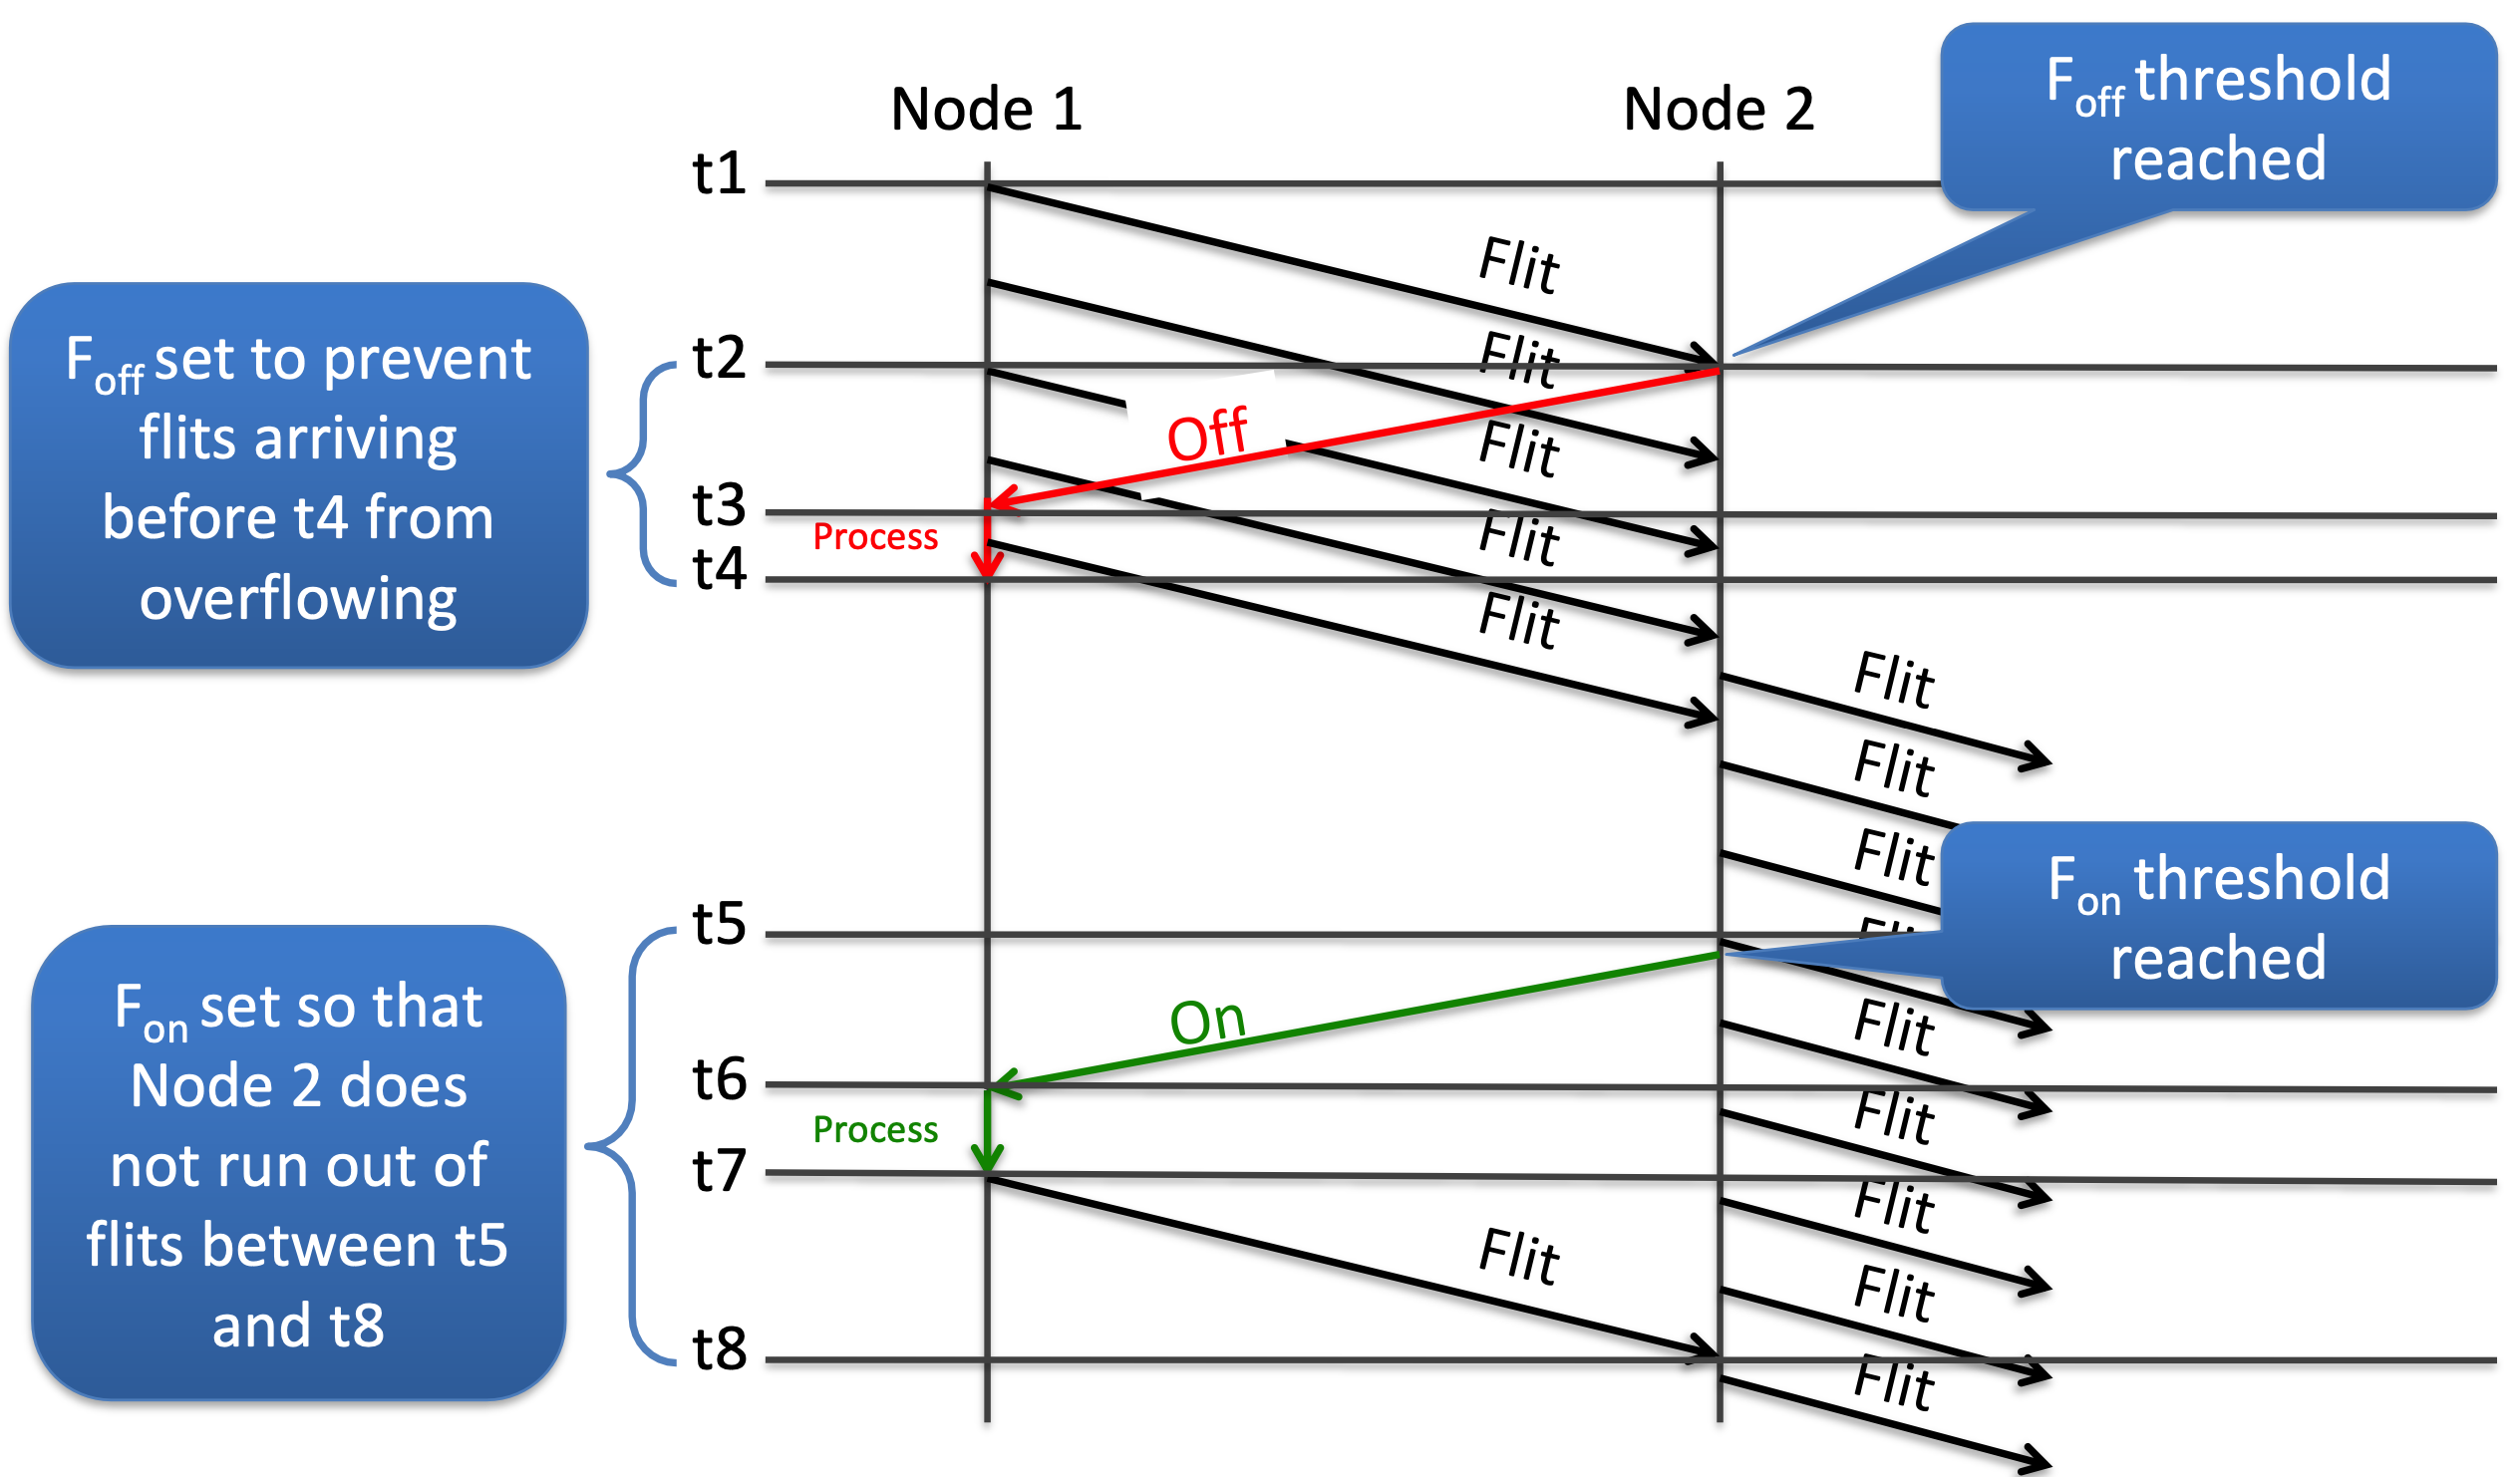
\includegraphics[width=.45\textwidth]{on_off.png}}
        \caption{On-Off timeline}
    \end{figure}     
\end{itemize}

\subsection{Interconnect Microarchitecture}

The following is a diagram of virtual channel router. Each input has a separate virtual channel.

\begin{figure}[H]
    \centering{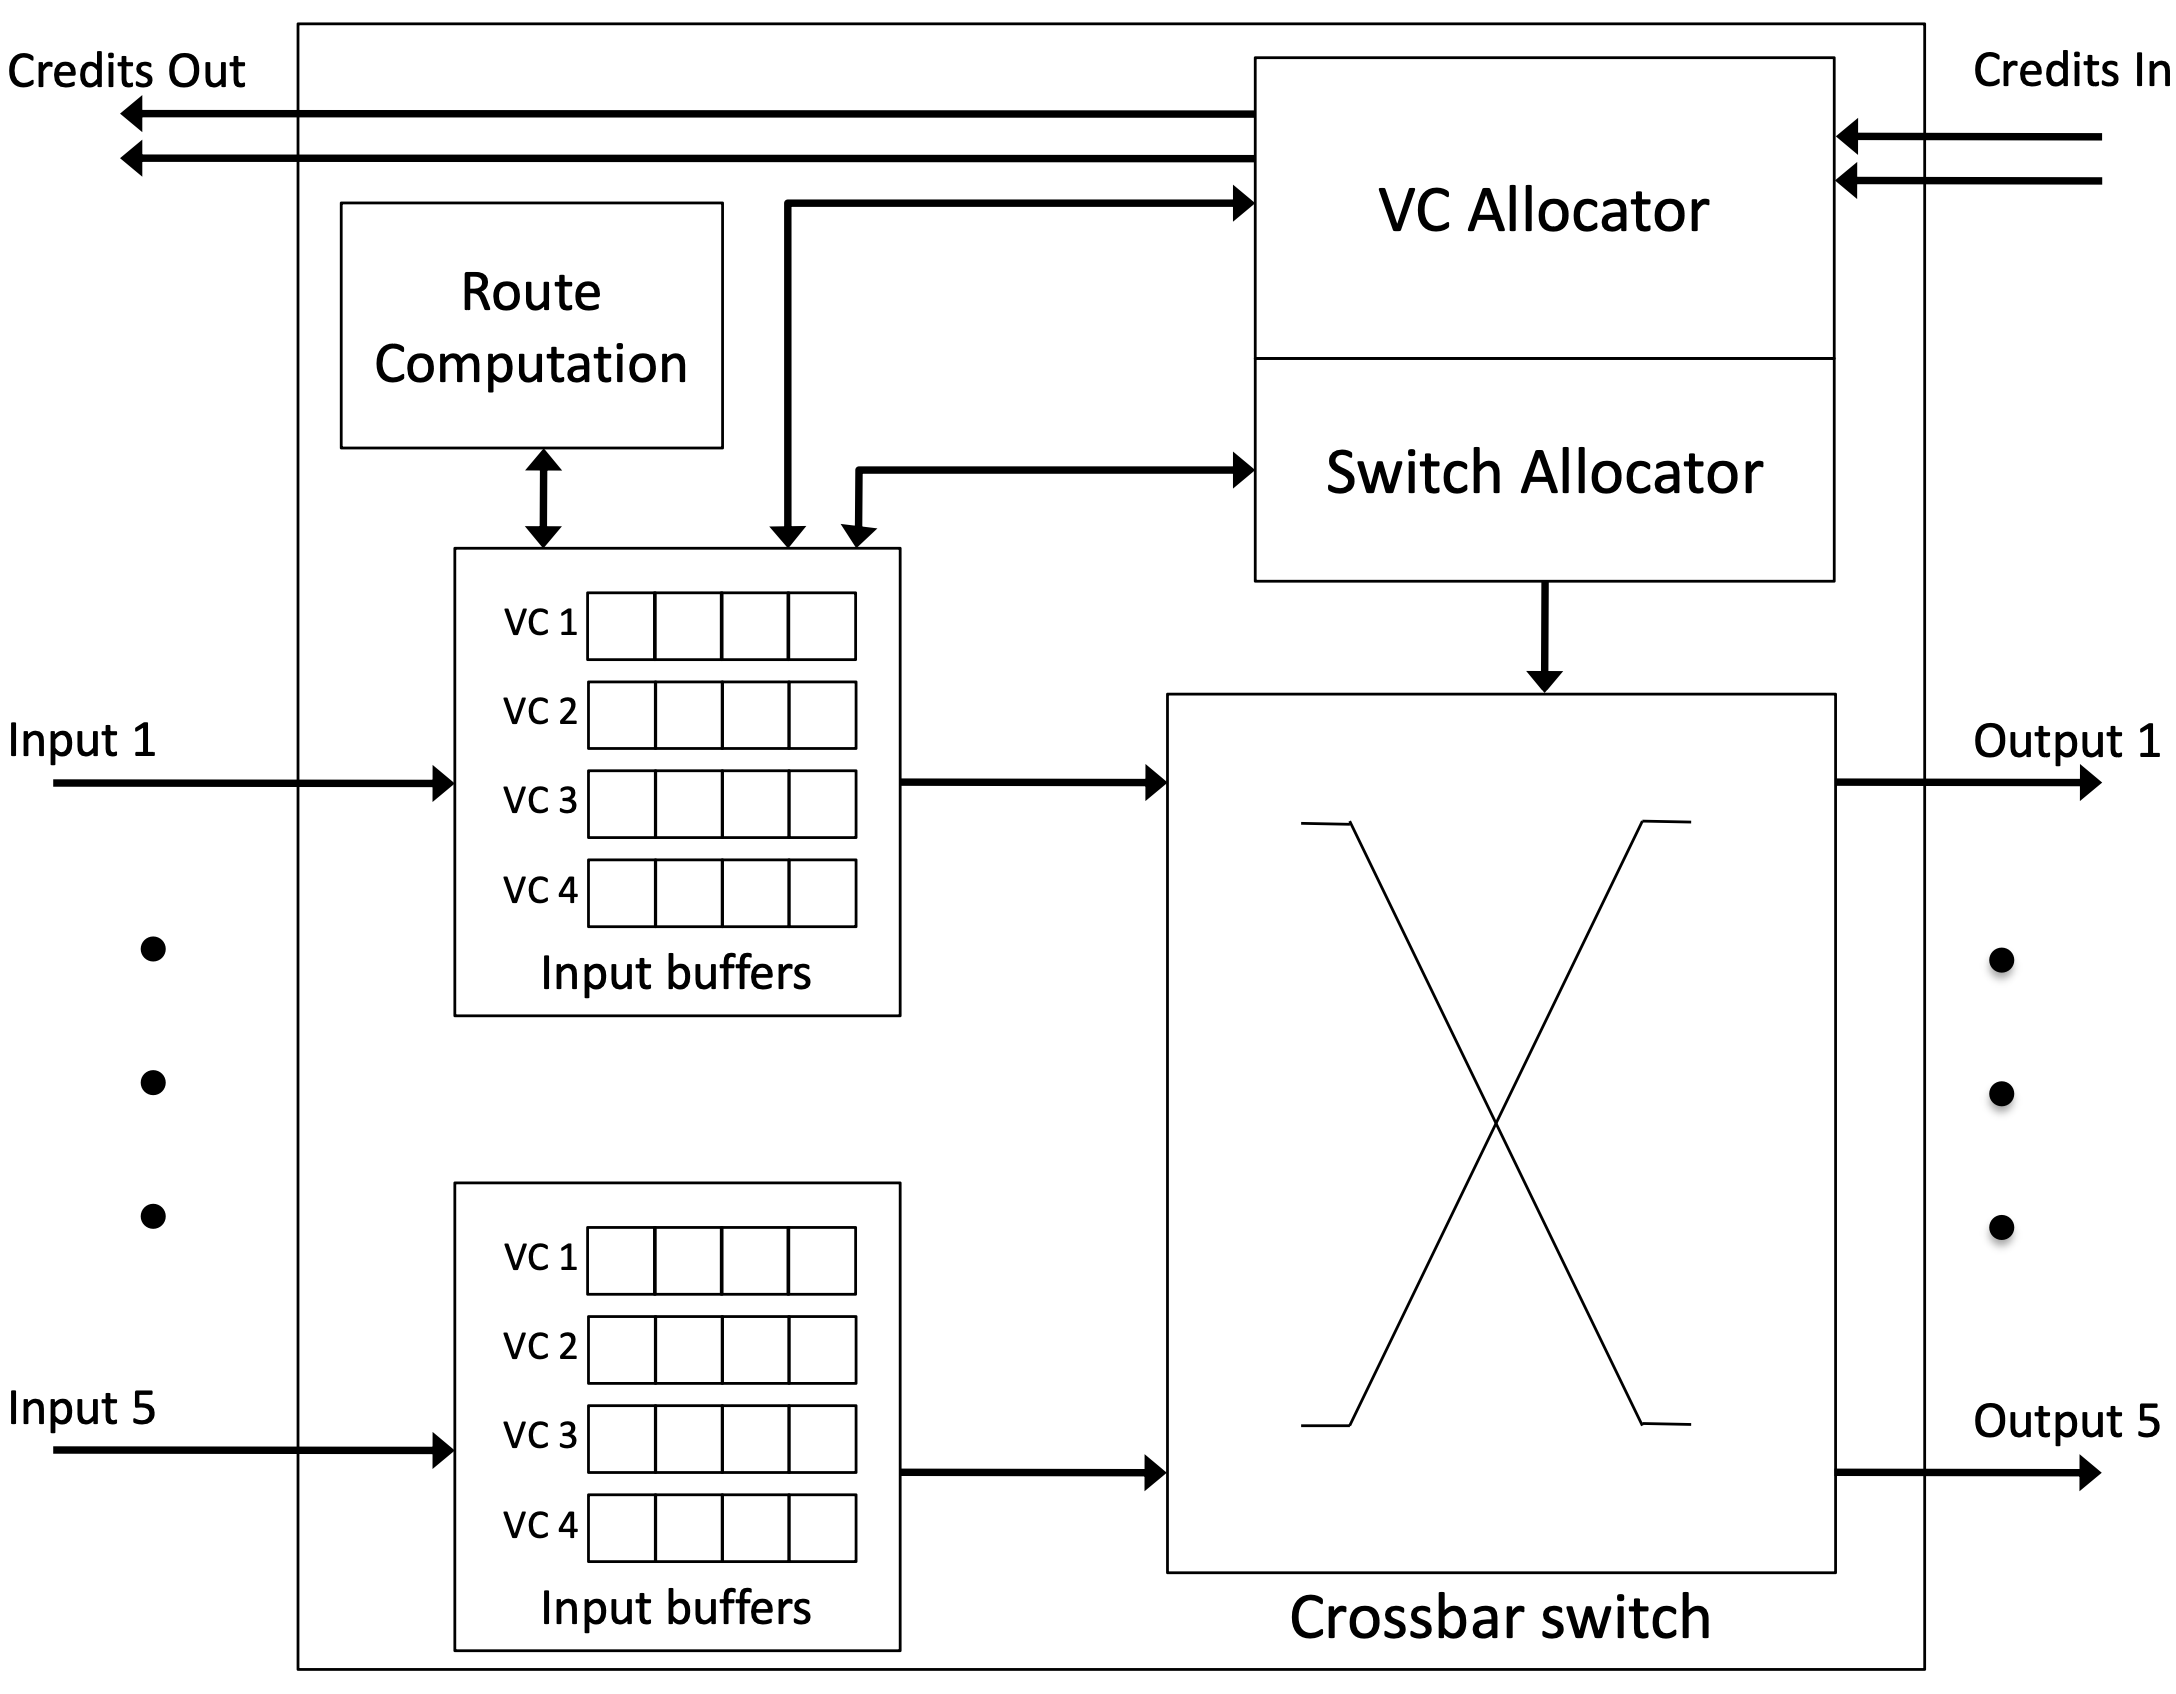
\includegraphics[width=.45\textwidth]{router_uarch.png}}
    \caption{Router $\mu$arch}
\end{figure}  

\subsubsection{Baseline router pipeline}
There are logical stages that fit into physical stages depending on frequency. Canonical pipeline stages include:
\begin{itemize}
    \item BW: Buffer write
    \item RC: Routing computation
    \item VA: Virtual channel allocation
    \item SA: Switch allocation
    \item ST: Switch traversal
    \item LT: Link traversal
\end{itemize}

\noindent\newline
RC/VA are performed once per packet. Flits after the head flit inherits the information.

\subsubsection{Pipeline optimizations}
\begin{itemize}
    \item Speculation: RC can overlap BW since RC for the next hop is independent of the remaining stages of the current hop. It is ok to do RC for the next hop in parallel at the current VA stage. Also one can assume VA is successful and can allow VA and SA in parallel. If VA is not successful, just repeat the VA/SA stage again.
    \item Bypassing: When there are no flits in the buffer, it is possible to enter ST speculatively (traverse the crossbar without entering the buffer). Before that, VC and RC is performed and crossbar is setup. If a output port conflict occurs, the flit is written to the buffer (BW) then performs SA.
\end{itemize}

\subsubsection{Buffer Organization}
Each input port can enter one of many queues depending which virtual channel is allocated. One can also use an unified buffer with multiple pairs of head/tail pointers that represent a VC. This is beneficial if one VC is less used than the other.

\subsubsection{Switch Organization}
For low frequency designs, we can direct inputs to $N$ outputs with $N$ multiplexers.

\noindent\newline
Another design is the crosspoint with each tri-state buffer inserted at every intersection. For multi-bit width connects, the switches are laid out diagonally.
\begin{figure}[H]
    \centering{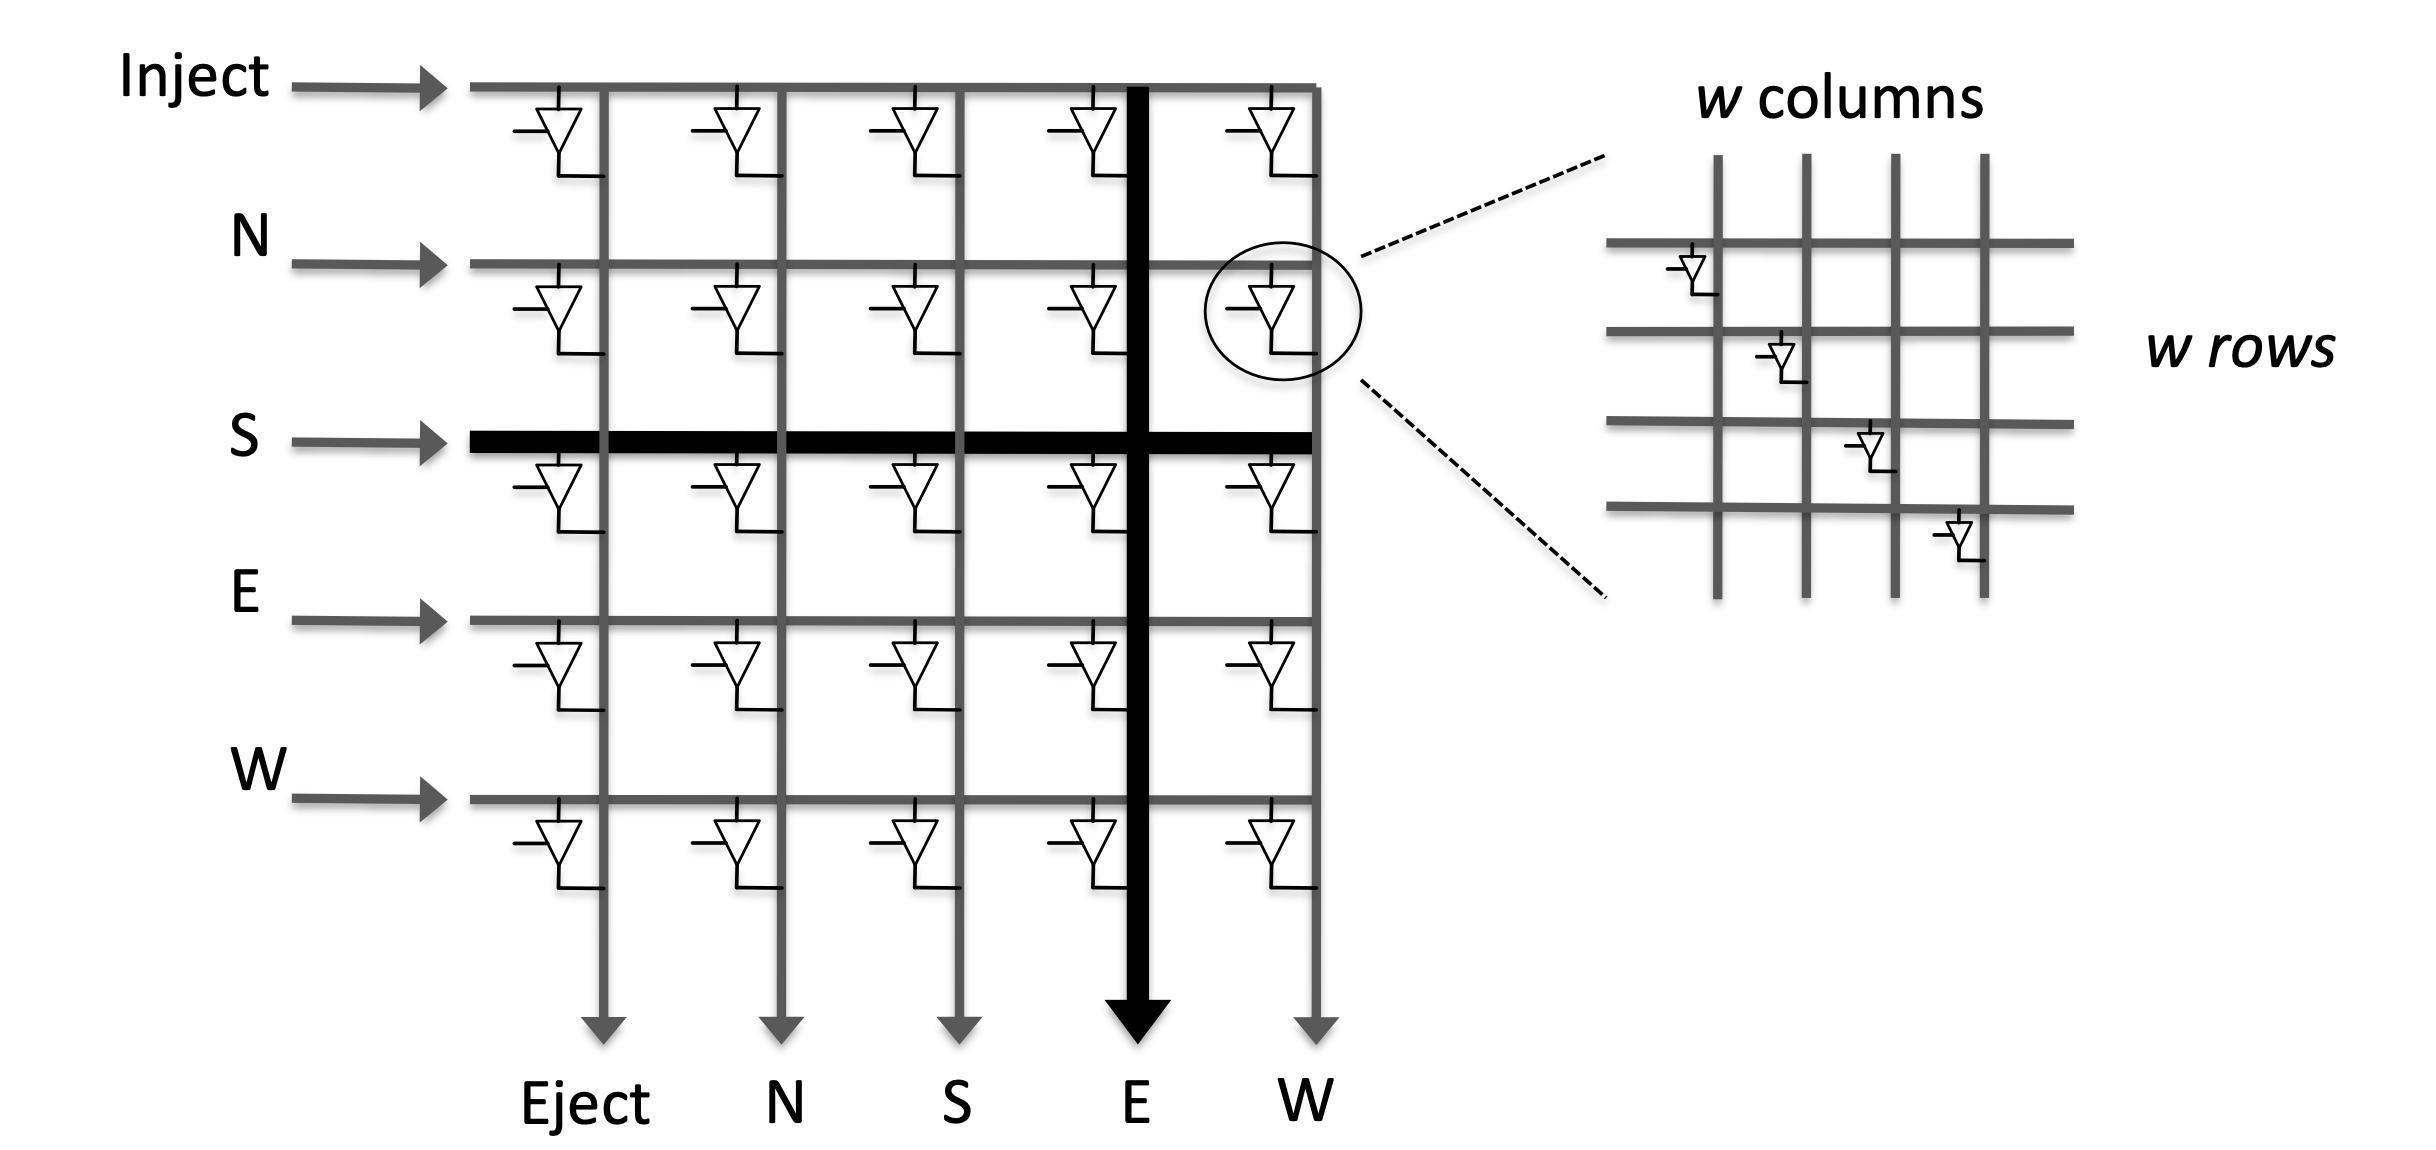
\includegraphics[width=.45\textwidth]{xpoint_sw.png}}
    \caption{Crosspoint switch}
\end{figure}  

\subsubsection{Crossbar speedup}
Crossbar speedup refers to input/output ports in the crossbar relative to the number of input/output ports of the router. With input speedup, the switch can take in flits in multiple VCs. With output speedup, it decreases the chance of flits conflicting to the same output with a cost of adding an output buffer.

\subsubsection{Arbiters and allocators}
In the VA stage, a VA allocator resolves contention for output VCs. In the SA stage, a SA allocator grants crossbar switch ports to input VCs. We can build allocators by stacking multiple arbiters. 
\medskip\noindent\newline
The separable switch allocator has 2 stages: In the first stage, each arbiter arbitrates the requester who won the bid for the resource. The second stage ensure that each requester would only receive one resource even if they have multiple bids won.
\begin{figure}[H]
    \centering{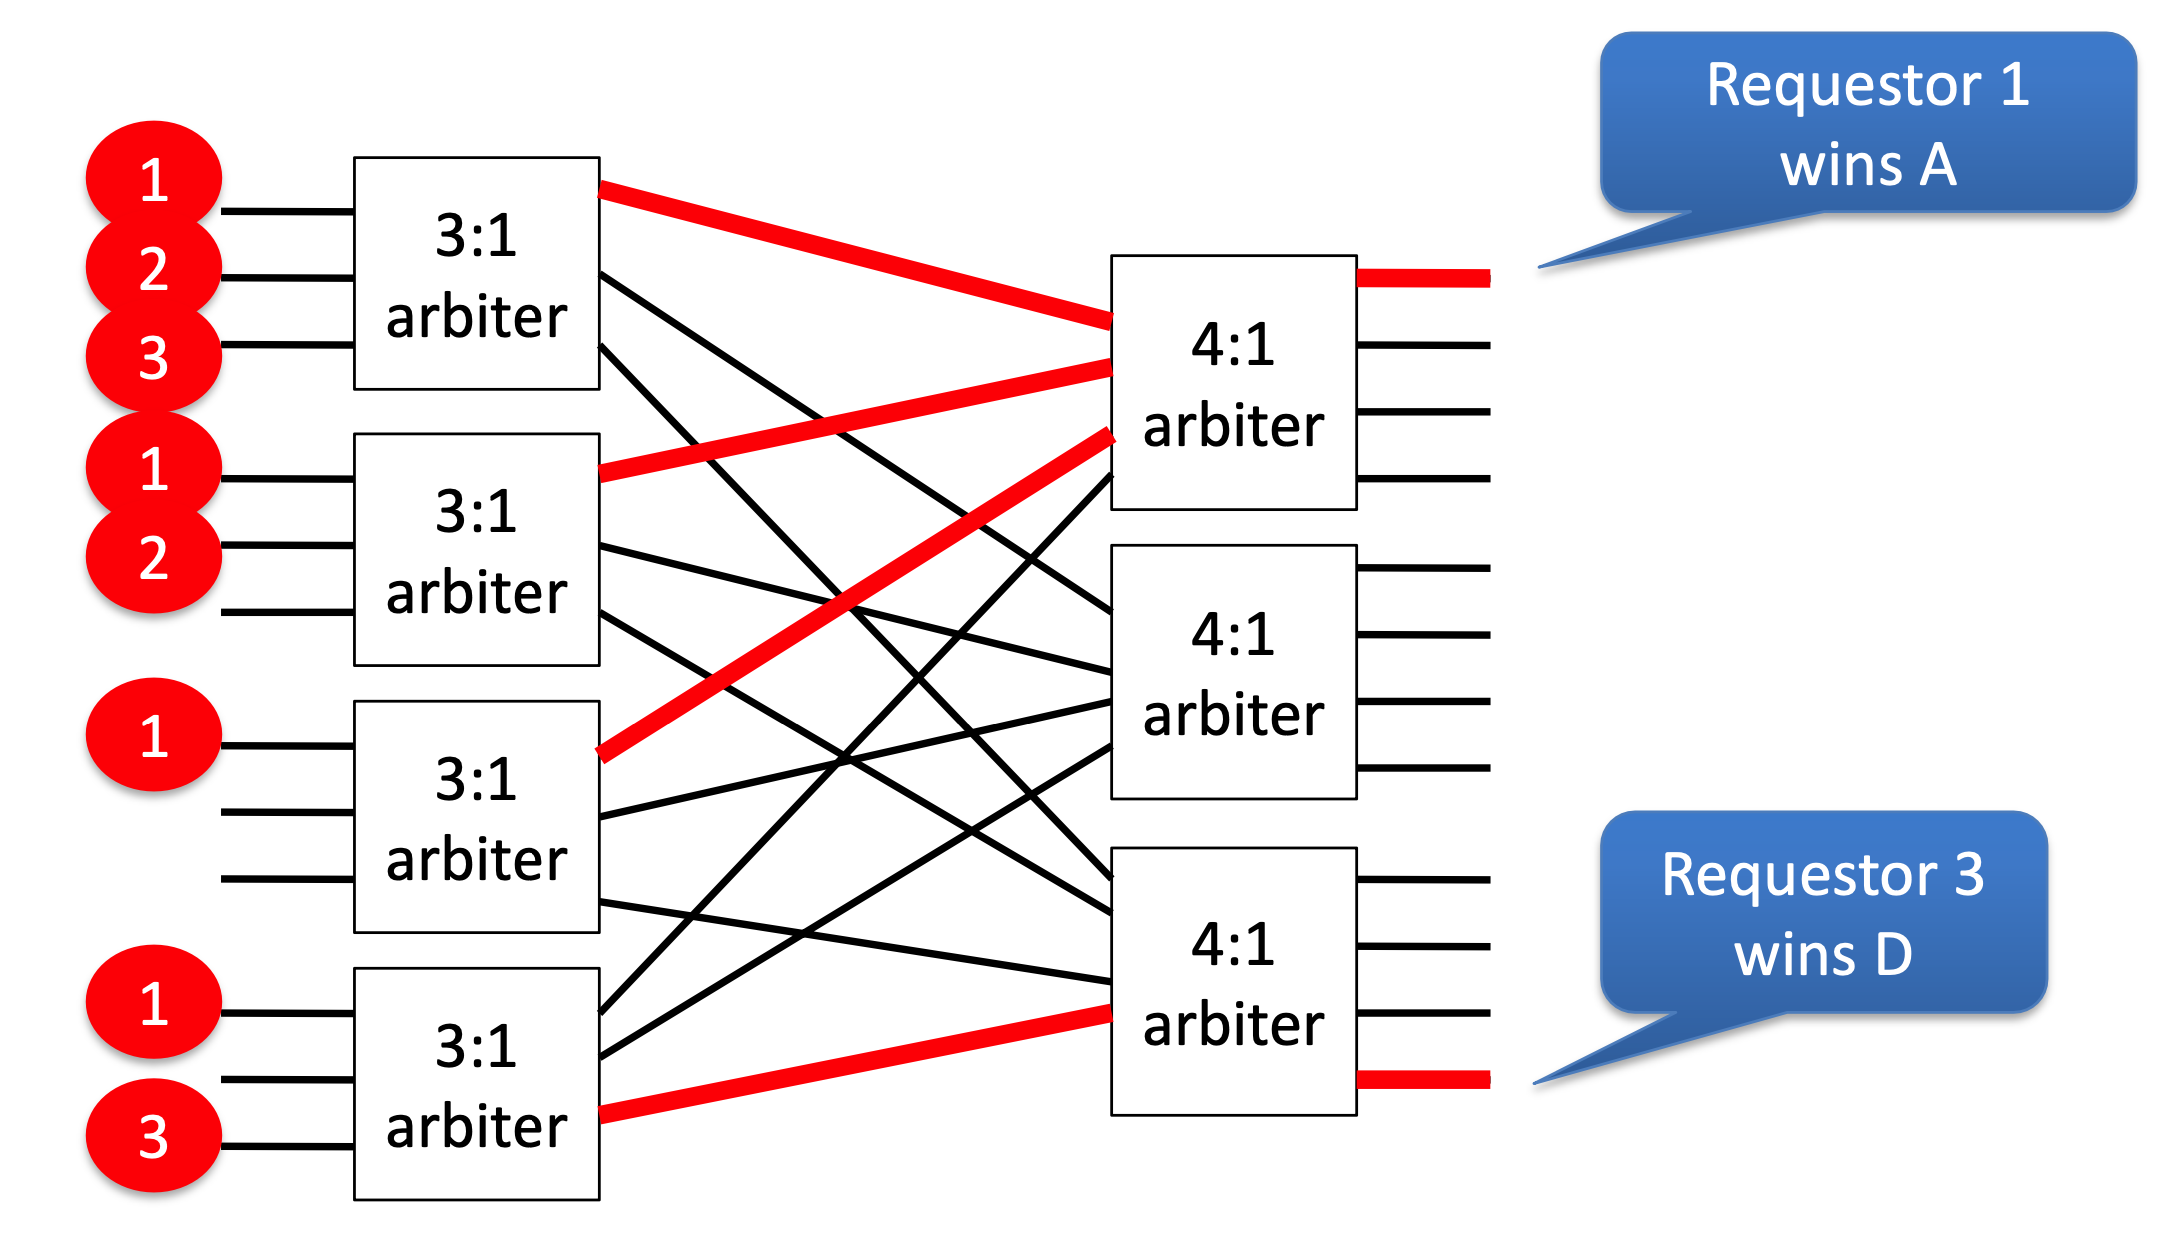
\includegraphics[width=.45\textwidth]{sep_allocate.png}}
    \caption{Separable allocator with 3 requesters and 4 resources (A/B/C/D)}
\end{figure}  

\section{Applications}

\subsection{Scientific and DB Applications}
Usually scientific applications have intensive computation with large datasets and predictable access patters. DB applications however, have huge data/instruction footprints with unpredictable sharing patterns.

\subsection{Standard Benchmarks}
There are 2 major flavors of benchmarks:
\begin{itemize}
    \item Online transaction processing (OLTP): Lots of small transactions with locking, concurrency and is memory bound.
    \item Decision support system (DSS): Consists of large read-only queries and is compute bound and highly parallel.
\end{itemize}

\subsection{Cloud Applications}
Scale-out workloads typically need:
\begin{itemize}
    \item Simple multithreaded cores
    \item Partitioned caches with no sharing
    \item Large on-chip instruction footprints
    \item Advanced prefetchers for irregular instruction access
\end{itemize}

\end{multicols*}
\end{document}

